\documentclass[12pt]{article}

\usepackage[margin=1in]{geometry} 
\usepackage{amsmath,amsthm,amssymb}
\usepackage{enumitem}
%\usepackage{minted}
\usepackage[unicode,hidelinks]{hyperref}
\usepackage{textcomp}
\usepackage{diagbox}
\usepackage[pdftex]{graphicx}
\usepackage{pdfpages}
\graphicspath{{images/}, {.}}

\usepackage{wrapfig}
\usepackage{cite} 

 
\usepackage{multirow}

\newcommand{\inp}[2]{\langle#1, #2\rangle}

\usepackage[margin=10pt,font=small,labelfont=bf]{caption}
\usepackage{subcaption}
\usepackage{longtable}
\usepackage{tabularx}
\usepackage{ltablex}

\usepackage{algorithm, algorithmicx, algpseudocode}

\usepackage{cmap}
\usepackage[T2A,T1]{fontenc} 
\usepackage[utf8]{inputenc} 
\usepackage[english,russian]{babel}

\newcommand{\N}{\mathbb{N}}
\newcommand{\Z}{\mathbb{Z}}
\newcommand*{\logequiv}{\ \Longleftrightarrow \ }
\newcommand*\mean[1]{\overline{#1}}
\renewcommand{\emptyset}{\varnothing}

%\renewcommand{\arraystretch}{1.5}
\linespread{1.3} % Полуторный интервал
%\pagestyle{plain}

\usepackage{booktabs}
\usepackage{makecell}

\usepackage{mathtools}

\usepackage{enumitem}
\AddEnumerateCounter{\asbuk}{\russian@alph}{щ}


%% compressed enumerate and itemize <<
\newenvironment{itemize*}%
{\begin{itemize}%
	\setlength{\itemsep}{0pt}%v
	\setlength{\parskip}{0pt}}%
{\end{itemize}}

\newenvironment{enumerate*}%
{\begin{enumerate}%
	\setlength{\itemsep}{0pt}%
	\setlength{\parskip}{0pt}}%
{\end{enumerate}}
%% >>

%% enumerate with russian numbering <<
\newenvironment{alphaenumerate*}
{\begin{enumerate}[label=(\asbuk*), ref=(\asbuk*)]
	\setlength{\itemsep}{0pt}
	\setlength{\parskip}{0pt}}
{\end{enumerate}}
%% >>


\newcommand{\hrefl}[1] {\texttt{\href{#1}{#1}}}
\newcommand{\children}[1] {\textsf{children}(#1)}

%% use alternative math letters and symbols << 
\renewcommand{\epsilon}{\varepsilon}
\renewcommand{\phi}{\varphi}
\let\smallcup\cup
\let\smallcap\cap
\renewcommand{\cup}{\bigcup}
\renewcommand{\cap}{\bigcap}
%% >>

%% clear page before each section <<
\let\oldsection\section
\let\oldsubsection\subsection
\renewcommand{\section}{\clearpage\oldsection}
\renewcommand{\subsection}{\clearpage\oldsubsection}
%% >>

\usepackage{cases}
\usepackage[geometry]{ifsym}

\newcommand{\itemizeBullet}{\scalebox{0.5}{\FilledSmallSquare}}
\renewcommand{\labelitemi}{\itemizeBullet}
\renewcommand{\labelitemii}{\itemizeBullet}
\renewcommand{\labelitemiii}{\itemizeBullet}

\begin{document}


% титульная страница
\includepdf{title.pdf}

% аннотация на русском
\begin{center}
	{\large Магистерская диссертация}
	\vspace{0.2cm}
	
	\textbf{\Large Метод обобщения в таксономиях и его применение}
	\vspace{0.4cm}
	
	{\large Власов А.С.}
	
\end{center}

\thispagestyle{empty}
\begin{abstract}
В работе рассматривается недавно предложенный в группе Б.Г. Миркина метод "<наиболее экономного"> обобщения в таксономиях. Предлагается модификация метода, использующая критерий максимального правдоподобия. Формируется необходимое математическое обеспечение, включая программу графического вывода для визуализации результатов. Метод применяется для анализа структуры массива 26000 журнальных публикаций в области Науки о данных за последние 20 лет с использованием имеющейся таксономии Науки о данных.  Метод аннотированного суффиксного дерева применяется для формирования коэффициентов релевантности между публикациями и ключевыми словами (терминальными темами таксономии). По этой информации формируются нечеткие кластеры ключевых слов, которые затем обобщаются с использованием разработанного матобеспечения. Вычисление вероятностей возникновения и потери смыслов в вершинах таксономии производится на основе результатов, полученных на 20\% случайных подмножествах публикаций. Результаты вычислений свидетельствуют о том, что критерии наибольшей экономии и максимального правдоподобия совместимы. Полученные кластеры и их обобщения в целом подтверждают сделанные ранее выводы (на основе массива 18000 статей), но значительно их детализируют.

\end{abstract}

% аннотация на английском
\clearpage
\renewcommand{\abstractname}{Abstract}
\begin{center}
	{\large Master' thesis}
	\vspace{0.2cm}
	
	\textbf{\Large Method for Appropriate Generalization in a Taxonomy}
	\vspace{0.4cm}
	
	{\large Vlasov A.S.}
	
\end{center}

\begin{abstract}
	This project considers a recently proposed method for maximally parsimonious generalization of fuzzy sets in taxonomies. The method is modified to the maximum likelihood criterion. A software is developed to support the computation, including a program for graphic visualization. The method applies to a collection of 26000 research papers in Data Science published over the past 20 years, using a taxonomy of Data Science developed earlier.   The method of Annotated Suffix Tree applies to compute relevance indices between the papers and keywords (topics corresponding to terminal nodes of the taxonomy). This data is used to find fuzzy clusters of keywords - these clusters then are parsimoniously generalized with the developed software. Probabilities of emergence and loss of meanings in the taxonomy nodes are computed based on results obtained at 20\% random samples of papers. Our computational results show that the criteria of maximum parsimony and maximum likelihood are compatible. The found clusters and their generalizations broadly support earlier conclusions made over results of similar analyses of a Springer's collection of 18000 papers, bringing in much more detail.
\end{abstract}
\newpage

% содержание (нумерация начинается здесь)
\setcounter{page}{1}
\tableofcontents
\newpage

% ==============================================================================
\section{Введение}

В последние годы задача автоматической структуризации и интерпретации текстовых коллекций является крайне актуальной. Количество текстовых интеллектуальных произведений, создаваемых людьми, неуклонно растет. Особенно ярко этот тренд проявляется в академической среде. К примеру, ежемесячное количество препринтов статей, выкладываемых авторами на крупнейший бесплатный архив электронных публикаций по физике, математике, астрономии, информатике и биологии \texttt{arxiv.org} на момент марта 2019 года составило более 12 тысяч\footnote{\texttt{https://arxiv.org/stats/monthly\_submissions}}. Такой бурный рост публикаций требует разработки инструментов, позволяющих исследователям автоматически анализировать и фильтровать этот огромный поток информации. В частности, интерес представляет задача \emph{обобщения} информации. Под обобщением понимается способность человека ставить в соответствие множеству некоторых концептов один или несколько более общих концептов, имеющих более крупную степень гранулярности. Один из методов обобщения --- индукция, то есть вывод некоторых общих закономерностей предметной области от частного к общему.

Большинство существущих подходов к структуризации текстовых коллекций не ставят своей целью их обобщение. Наиболее популярные методы структурирования в настоящее время --- кластер-анализ \cite{mirkin2005clustering} и тематическое моделирование \cite{blei2003latent, Papadimitriou:1998:LSI:275487.275505}. Оба подхода используют признаки того же уровня гранулярности, что и отдельные слова или короткие фразы из текстов, поэтому с их помощью задачу обобщения решить не удается.

Тем не менее, исследования иерархической структуры определений и понятий активно ведутся. Активно ведется разработка таксономий, в особенности таких, которые отражают отношения гипонимии/гиперонимии (см. \cite{snow2006semantic}). В их числе присутствуют попытки автоматического построения таксономий на основе коллекции ключевых словосочетаний \cite{Osborne2012, Osborne2015}, а так же улучшения существующих таксономий добавлением новых, еще только зарождающихся понятий \cite{vedula2018enriching}.

Другим направлением исследований является суммаризация текстов. Как правило, алгоритмы суммаризации согласно определенным правилам выделяют из текста ключевые словосочетания или предложения. Одним из подходов является выделение из текста фраз, заданных некоторыми шаблонами, к примеру тройками субъект-глагол-объект (subject-verb-object, SVC).

Подход к обобщению, используемый в этой работе, основан на разработанном Б.Миркиным и его соавторами в \cite{mirkin2003algorithms, mirkin2006aggregating, mirkin2018preprint} методе наибольшей экономии. Обобщение в нем рассматривается как отношение включения одного понятия в другое: если понятие A --- обобщение понятия B, то B является частным случаем понятия A. В качестве обобщаемого множества объектов используется нечеткое множество, заданное на листьях таксономии компьютерных наук ACM Computing Classification System 2012 \cite{associationforcomputingmachinery}. Обобщением в данном случае будет являться множество вершин таксономии более высокого уровня.

Недавно предложенный метод обобщения был применен Д.Фроловым и Б.Миркиным к задаче анализа тенденций в области науки о данных \cite{mirkin2018preprint}. Целью магистерской диссертации является продолжение, уточнение и улучшение этой работы. Для достижения цели диссертации были поставлены следующие цели:

\begin{itemize*}
	\item Изучить и освоить метод обобщения с критерием наибольшей экономии.
	\item Модифицировать метод обобщения с использованием критерия максимального правдоподобия.
	\item Подготовить текстовую коллекцию аннотаций научных статей и таксономию.
	\item Построить матрицу релевантности текстов аннотаций к темам исследований, заданным листьями таксономии.
	\item Преобразовать матрицу релевантности текстов в матрицу корелевантности тем исследований.
	\item Применить метод нечеткой кластеризации к матрице корелевантности и получить нечеткие кластеры над множеством тем исследований.
	\item Обобщить полученные кластеры с помощью алгоритма, использующего метод наибольшей экономиии и алгоритма, использующего метод максимального правдоподобия.
	\item Провести анализ результатов обобщения и сравнить методы между собой.
	\item Сделать выводы относительно современных тенденций в области наук о данных.
\end{itemize*}

По сравнению с \cite{mirkin2018preprint} эксперимент, описанный в данной магистерской диссертации, имеет следующие преимущества:

\begin{itemize*}
	\item Использован метод обобщения с критерием максимального правдоподобия, проведено сравнение результатов с полученными методом наибольшей экономии.
	\item Использовано текстовая коллекция большего размера (26 000 статей против 18 000).
	\item  Для оценки релевантности строк к тексту использован метод аннотированного суффиксного дерева на 5-граммах (против 3-грамм в \cite{mirkin2018preprint}). В \cite{Chernyak_2015} показано, что это значение оптимально.
	\item Получено семь интерпретируемых тематических кластеров (против трех в \cite{mirkin2018preprint}).
	\item Построена и проанализирована диаграмма взаимодействия тематических кластеров.
	\item Выводы о тенденциях в науках о данных расширены и обобщены.
\end{itemize*}


Структура работы организована следующим образом. В разделе 2 формально ставится задача обобщения нечеткого множества на таксономии и приводятся две модификации алгоритма обобщения.  В разделе 3 описан ход эксперимента: подготовка данных, методы вычисления матрицы релевантности и корелевантности, метод кластеризации, описано разработанное ПО. В конце раздела представлены результаты эксперимента в виде таблиц и графиков. Результаты проанализированы и сделаны выводы.


% ==============================================================================
\section{Метод обобщения}

% ------------------------------------------------------------------------------
\oldsubsection{Модель обобщения в таксономии}

С математической точки зрения таксономия --- это корневое дерево, вершины которого аннотированы различными понятиями (темами) предметной области. Рассмотрим следующую задачу. Дано нечеткое множество $S$, элементы которого являются листьями таксономии. Необходимо найти вершину более высокого уровня $t(S)$ (головное понятие, головная тема, head subject), которая как можно более плотно покрывает множество $S$. Подобная задача "<подъема"> --- это математически заданная модель способности человека к обобщению информации. При этом обобщаемые концепты заданы нечетким множеством на листьях таксономии.

Формальная постановка задачи обобщения разработана Б.Миркиным, Т.Феннером и др. в \cite{mirkin2003algorithms} в приложении к эволюционной биологии. Была сформулирована и предпринята попытка решения задачи определения оптимального сценария переноса (потери и приобретения) генов на эволюционном дереве организмов. Дальнейшее развитие метод получил в \cite{mirkin2006aggregating}, где применялся так же к задаче биологии, и в \cite{mirkin2018preprint}, где метод был применен к задаче структуризации и концептуализации коллекции научных текстов.
%%%is not as simple ...?

Приведем основные понятия, необходимые для постановки задачи. При подъеме множества $S$ может возникнуть два типа ошибок --- пробелы (gap) и выбросы (offshoot). На рис. \ref{fig:gap_offshoot_example} показан пример обобщения множества, состоящего из листьев таксономии и выделенного серым цветом, одним головным понятием. На рисунке отражены два типа ошибок:
\begin{itemize*}
	\item Пробел ---  лист, не принадлежащий исходному множеству, но попавший в часть дерева, лежащую под головным понятием.
	\item Выброс --- лист, который остался непокрытым головным понятием несмотря на то, что он принадлежал исходному множеству. 
\end{itemize*} 

\begin{figure}
\centering
\includegraphics[width=0.5\linewidth]{images/gap_offshoot_example}
\caption{Обобщение множества, выделенного серыми цветом на таксономии. Указано головное понятие и два типа ошибок.}
\label{fig:gap_offshoot_example}
\end{figure}

В терминах задачи классификации пробел --- это  ошибка первого рода (false positive), выброс --- ошибка второго рода (false negative). 

Один из способов обобщить множество --- взять в качестве головного понятия последнюю (наиболеее глубокую) вершину, которая является предком для каждой из вершин во множестве. Несмотря на простоту этого метода, он не всегда будет оптимальным, т.к. не принимает в расчет возможность наличия аномальных или ошибочных элементов в исходном множестве и, зачастую, приводит к большому количеству пробелов. Таким образом, хороший алгоритм обобщения должен решать многокритериальную задачу, которая тем или иным образом минимизирует количество элементов обобщения: головных понятий, пробелов и выбросов. Штрафы за наличие этих элементов должны учитывать экспертное мнение исследователя. 

Согласно \cite{mirkin2018preprint} введем следующие определения:
\begin{itemize*}
	\item $T$ --- направленное корневое дерево, вершины которого аннотированы темами предметной области, а ребра выражают отношение включения.
	\item $I$ --- множество \textit{листьев} дерева $T$.
	\item $\chi(t)$ --- множество \textit{детей} вершины $t$. Вершина $t$ является \textit{ребенком} вершины $t'$, если существует ребро от $t'$ к $t$. Обратно: $t$ --- \textit{родитель} $t'$, если существует ребро от $t$ к $t'$.
	\item $T(t)$ --- \textit{поддерево} вершины $t$ (сама вершина и все ее потомки).
	\item $I(t)$ --- множество листьев поддерева $T(t), \ t\in T\setminus I$ (\textit{листовой кластер}).
	
	\item $S=\{u(i)\geq0,\forall i\in I\}$ --- \textit{нечеткое множество} на $I$.
	\item $S_u=\{i\in I: u(i)>0\}$ --- \textit{основа} нечеткого множества $S$.
\end{itemize*}

Введем понятия, необходимые для формального определения пробелов, выбросов и головных тем: 
\begin{itemize*}
	\item $t\in T$ называется $u$-\textit{нерелевантной}, если $I(t) \smallcap S_u=\emptyset$ (т.е. ее листовой кластер не пересекается с основой нечеткого множества).
	Все потомки $t$ так же будут являтся $u$-нерелевантными.
	\item $g\in T(h)\setminus\{h\}$ называется $h$-\textit{пропуском}, если это максимально $u$-нерелевантная вершина (в том смысле, что ее родитель не является $u$-нерелевантным). 
	%%% что-то объяснить!
	\item $G(h)$ --- множество всех $h$-пропусков.
	\item $i\in S_u: i\notin I(h)$ называется $h$-\textit{выбросом} (лист, который не покрыт вершиной $h$).
	\item $S_u \setminus I(h)$ --- множество всех $h$-выбросов.
\end{itemize*}

Т.к. никакая таксономия не может идеально описать все отношения в реальном мире, некоторые нечеткие множества тем могут относиться к более широким понятиям, которые не отражены в используемой таксономии. В этом случае для того, чтобы покрыть все вершины наиболее оптимальным способом, может понадобиться больше одного головных понятия. Исходя из этих соображений, дадим еще несколько определений:

\begin{itemize*}
	\item $H=\{t\in T\}$ называется $u$-\textit{покрытием}, если выполняются следующие условия:
	\begin{enumerate*}
		\item $S_u\subseteq \cup_{h\in H}I(h)$ ($H$ покрывает $S_u$),
		\item $\forall h, h' \in H: h\neq h' \implies I(h)\cap I(h') = \emptyset$ (множества листовых кластеров для любых вершин из $H$ не пересекаются).
	\end{enumerate*}
	\item $\textsf{heads}(H)=H\setminus I$ --- множество \textit{головных понятий} (внутренних вершин $H$).
	\item $\textsf{offshoots}(H) = H\smallcap I$ --- множество \textit{выбросов} (листовых вершин $H$).
	\item $\textsf{gaps}(H) = \cup_{h\in H-I}G(h) $  --- множество \textit{пробелов} (объединение множества $h$-пробелов для вершин из $H$).
\end{itemize*}

В общем случае элементы нечеткого множества $S$ объединены некоторой темой (понятием). Элементы этого множества соответствуют этому понятию, являются его подмножеством. Тогда, если вершина принадлежит множествам $\textsf{heads}(H)$ или $\textsf{offshoots}(H)$, то можно говорить о \textit{приобретении головного понятия}. Аналогично, если вершина принадлежит множеству $\textsf{gaps}(H)$, то говорят о \textit{потере головного понятия}. Со множеством $H$ необходимо ассоциировать некоторую функцию потерь, которая включает в себя штрафы за избыточное количество головных тем, выбросов и пробелов. Положим:

\begin{itemize*}
	\item $\lambda\geq1$ --- штраф за пробел.
	\item $\gamma\geq0$ --- штраф за выброс.
	\item Штраф за введение нового головного понятия равен 1.
\end{itemize*} 
%%% пример выбора?

Очевидно, что значение штрафа, ассоциированного с вершиной $h\in H$ должно учитывать значения функции принадлежности $u$ всех вершин листового кластера $I(h)$: чем они меньше, тем меньше штраф. По этой причине необходимо расширить область значений функции принадлежности $u(\cdot)$ на все вершины дерева. Это может быть достигнуто с помощью некоторой аггрегирующей функции $f$:
\begin{equation}
	u(t) = f(\{u(i),i\in I(t)\}), \ t\in T-I.
\end{equation}
Для случая, когда значения функции принадлежности нормированы так, что сумма их квадратов равна единице ($\sum_{i\in S_u}u(i)^2=1$), предлагается следующая функция аггрегации:
\begin{equation}
	u(t) = \sqrt{\sum_{i\in I(t)}u(i)^2}, \quad  t\in T\setminus I.
	\label{eq:u_extend}
\end{equation} %% TODO подумать почему?
Мотивация использования такой функции аггрегации следующая. Значения функции принадлежности с квадратичной нормализацией можно рассматривать, как вклады индивидуальных элементов в общую "<массу"> кластера. Естественно предположить, что функция аггрегации должна наследовать это свойство так, чтобы вклад каждой из внутренних вершин был равен суммарному вкладу ее листового кластера. Выбранная функция аггрегации удовлетворяет этому условию.

Кроме этого, несмотря на то, что все пробелы обладают значением принадлежности $u$, равным нулю, мы можем считать некоторые пробелы более критичными, чем другие. Для этого определим значение \textit{"<важности пробела">} $v(g)$. Интуитивно понятно, что чем меньше значение принадлежности родителя вершины-пробела, тем менее значим для нас пробел. Авторами \cite{mirkin2018preprint} предложено следующее формальное определение важности пробела:
\begin{equation}
	v(g)=u(\textsf{parent}(g)), \quad g\in T,
	\label{eq:gap_importance}
\end{equation}
где $\textsf{parent}(g)$ --- вершина-родитель $g$.

Исходя из всех данных выше определений и соображений в следующем разделе определим конкретную функцию потерь для данного множества $H$ и приведем алгоритм нахождения оптимального $H$, соответствующего минимуму этой функции.


% ------------------------------------------------------------------------------
\subsection{Критерий наибольшей экономии и метод}

Исходя из принципа максимальной экономии (Maximum Parsimony), популярному в биоинформатике \cite{robinson2011introduction}, оптимальное множество $H$ должно минимизировать количество элементов обобщения: головных понятий, выбросов и пробелов. Этот подход можно расширить, используя не количество элементов, а значения их функции принадлежности, взвешенные соответствующими штрафными коэффициентами. Авторами \cite{mirkin2018preprint} предложена следующая функция потерь для $u$-покрытия $H$, учитывающая это соображение:

\begin{equation}
	p(H)=\sum_{h\in \textsf{heads}(H)}u(h) + \sum_{h\in \textsf{heads}(H)}\sum_{g\in G(h)}\lambda v(g) + \sum_{h\in \textsf{offshoots}(H)}\gamma u(h).
	\label{eq:pars_criterion}
\end{equation}
В предложенной функции потерь первое слагаемое --- штраф за введение новых головных понятий, второе --- штраф за пробелы, третье --- штраф за выбросы.

Приведем алгоритм, разработанный в \cite{mirkin2018preprint}, позволяющий найти $H$, соответствующее глобальному минимуму критерия \eqref{eq:pars_criterion}. Для его работы необходимо подготовить дерево таксономии: удалить все не-максимальные $u$-нерелевантные вершины (потомки $h$-пропусков), каждой из вершин сопоставить множество пропусков $G(t)$ и суммарную важность пропусков:
\begin{equation}
	V(t)=\sum_{g\in G(t)}v(g).
	\label{eq:sum_gap_importance}
\end{equation}

Далее будем считать, что дерево уже подготовлено и все его вершины аннотированы величинами $u(t), \ G(t), \ v(t), \ V(t)$. Для каждой вершины алгоритм ParGenFS рекурсивно (снизу вверх, начиная с листьев) вычисляет следующие величины:
\begin{itemize*}
	\item $H(t)$ --- вершины, в которых головное понятие было приобретено (головные вершины или выбросы);
	\item $L(t)$ --- вершины, в которых головное понятие было потеряно (пропуски);
	\item $p(t)$ --- величина штрафа, связанного с множеством $H(t)$.
\end{itemize*}
Предполагается, что в вершине \emph{не может} произойти приобретения понятия после того, как оно уже было потеряно в одном из предков данной вершины.

В базовом случае, когда $t$ --- лист дерева:

\begin{itemize*}
	\item Если $t\notin S_u$, то $H(t)=\emptyset, \ L(t)=\emptyset,\ p(t)=0$;
	\item Если $t\in S_u$, то $H(t)=\{t\}, \ L(t)=\emptyset,\ p(t)=\gamma u(t)$;
\end{itemize*}

Для того, чтобы вычислить $H(t)$ и $L(t)$ для любой из внутренних вершин, необходимо рассмотреть два случая:
\begin{alphaenumerate*}
	\item\label{enum:head_gained} Головное понятие было приобретено в $t$, тогда:
	\begin{equation}
		\begin{aligned}
			H(t) &=\{t\},\\
			L(t)&=G(t), \\
			p(t)& = u(t) + \lambda V(t).
		\end{aligned}
	\end{equation}
	\item Головное понятие \emph{не было} приобретено в $t$, тогда:
	\begin{equation}
		\begin{aligned}
			H(t)=&\cup_{w\in \chi(t)} H(w),\\
			L(t)=&\cup_{w\in \chi(t)} L(w), \\
			p(t) =& \sum_{w\in \chi(t)}p(w).
		\end{aligned}
	\end{equation}
\end{alphaenumerate*}

Вершине присваивается тот набор параметров, для которого значение $p(t)$ меньше. В случае, если в обоих случаях значения $p(t)$ совпадают, берется любой из наборов, пусть это будет \ref{enum:head_gained}. В случае, если $t^*=\textsf{root}(T)$ --- корень дерева, то работа алгоритма закончена и возвращается результат: $H(t^*)$ --- множество головных понятий и выбросов, $L(t^*)$ --- множество пробелов и $p(t^*)$ --- значение штрафной функции. Алгоритм \ref{algo:pargenfs} формализует описанные шаги вычислений.

\begin{algorithm}
	\floatname{algorithm}{Алгоритм}
	\caption{ParGenFS (Parsimonious Generalization of Fuzzy Sets)}\label{algo:pargenfs}
	\vspace{5pt}
	\textbf{Входные данные:} Подготовленное дерево $T$, вершины которого аннотированы величинами $u$, $G$, $v$, $V$.  \\
	\textbf{Выходные данные:} $H, \ L, \ p$ 
	
	\newcommand{\child}{\textsf{w}}
	\newcommand{\node}{\textsf{t}}
	\begin{algorithmic}[1]
		\For {$\node$ in $\textsf{ReverseLevelOrderTraversal}^\nabla(T)$}\vspace{2pt}
			\If {$\node$ is leaf}
				\If {$\node.u>0$}
					\State $\node.H \gets \{\node\}$
					\State $\node.L \gets \emptyset$
					\State $\node.p \gets \gamma\cdot \node.u$	
				\Else
					\State $\node.H \gets \emptyset$
					\State $\node.L \gets \emptyset$
					\State $\node.p \gets 0$
				\EndIf
			\Else
				\If {$\node.u + \lambda\cdot \node.V \leq \sum_{\child\in \chi(\node)}\child.p$}
					\State $\node.H \gets \{\node\}$
					\State $\node.L \gets \node.G$
					\State $\node.p = \node.u + \lambda\cdot \node.V$
				\Else
					\State $\node.H \gets \cup_{\child\in \chi(\node)} \child.H$
					\State $\node.L \gets \cup_{\child\in \chi(\node)} \child.L$
					\State $\node.p = \sum_{\child\in \chi(\node)}\child.p$
				\EndIf
			\EndIf
		\EndFor
		\State \Return { $\textsf{root}(T).H, \ \textsf{root}(T).L, \textsf{root}(T).p$ }
	\end{algorithmic}
	{\footnotesize$~^\nabla$Обратный обход дерева в порядке уровней: начинают с листьев, затем переходят к вершинам на один уровень выше листьев, далее на два уровня и т.д.}
\end{algorithm}

Авторами \cite{mirkin2018preprint} доказано, что результатом работы алгоритма ParGenFS действительно является $u$-покрытие $H$, глобально минимизирующее функцию потерь \eqref{eq:pars_criterion}.

В следующем разделе приведем модификацию экономичного метода обобщения, которая строит $u$-покрытие $H$ исходя из вероятности возникновения такого сценария, в котором потери и приобретения головных тем произошли в пробелах и в головных понятиях $H$ соответственно.

% ------------------------------------------------------------------------------
\subsection{Критерий максимального правдоподобия и метод}

Для того, чтобы перейти от эвристического критерия наибольшей экономии \eqref{eq:pars_criterion} к более естественному критерию максимального правдоподобия, введем понятие \textit{сценария}, ассоциированного с произвольным $u$-покрытием $H$. Сценарий --- это множество событий $E$, ассоциированных с каждой из вершин дерева $T$. Каждой вершине соответствует ровно одно событие $e_t$. Сценарий для вершины $t\in T$ строится по следующим правилам:

\begin{itemize*}
	\item Если $t\in H$, тогда  в $t$ произошло приобретение головной темы (gain, G).
	\item Если $t\in \textsf{gaps}(H)$, тогда в $t$ произошла потеря головной темы (loss, L).
	\item Если $t\notin H \smallcup \textsf{gaps}(H)$, тогда в $t$ не произошло ни приобретения, ни потери головной темы. В этом случае считаем, что вершина содержит "<пустое событие">, при котором потомкам передается головная тема, если она изначально была унаследована (pass, P).
	\item В $t=\textsf{root}(T)$ произошла потеря головной темы.
\end{itemize*}
Таким образом, формальное определение сценария:

\begin{equation}
	Sc(H) = \{e_t(H),\forall t\in T\}, \quad e_t(H) \in \{G, L, P\}.
\end{equation}

Кроме этого, с каждой из вершин необходимо ассоциировать априорные вероятности приобретения ($p^G$) и потери ($p^L$) головной темы. Эти вероятности можно получить, построив обобщение множества нечетких кластеров и вычислив частотности событий для каждой вершины:

\begin{equation}
	\begin{gathered}
		p_t^L = \frac{\#[\text{потерь в вершине }t]}{\#[\text{кластеров}]}, \\
		p_t^G = \frac{\#[\text{приобретений в вершине }t]}{\#[\text{кластеров}]},
	\end{gathered}
	\label{eq:loss_gain_freq}
\end{equation}
где $\#[X]$ --- количество элементов во множестве $X$. Задача нахождения оптимального $u$-покрытия для данного дерева $H$ и нечеткого кластера $S$ c функцией принадлежности $u$ в данных терминах формулируется следующим образом:

\begin{equation}
	H = \arg\max_H p(Sc(H)).
\end{equation}

Количество возможных сценариев для дерева $T$ экспоненциально велико (порядка $3^n$, где $n$ --- число вершин дерева), поэтому решить эту оптимизационную задачу точно не представляется возможным. Для того, чтобы получить ее субоптимальное решение, используем рекурсивный алгоритм, который жадным образом строит наиболее вероятный сценарий. Рассмотрим два случая:
\begin{enumerate*}
	\item Вершина $t$ \emph{унаследовала} головное понятие от своего родителя, тогда возможны два события:
	\begin{alphaenumerate*}
		\item\label{enum:a} Потеря $L$ головного понятия в $t$. Вероятность этого равна $$p_t^L\prod_{w\in\children{t}}p_w^N,$$ где $p_w^N$ --- вероятность того, что $w$ \emph{не унаследовала} от $t$ головное понятие.
		\item\label{enum:b} Потери не происходит (событие pass). Вероятность этого равна $$(1-p_t^L)\prod_{w\in\children{t}}p_w^I,$$ где $p_w^I$ --- вероятность того, что $w$ \emph{унаследовала} от $t$ головное понятие.
	\end{alphaenumerate*}
	В этом случае выбирается наиболее вероятное событие из \ref{enum:a} и \ref{enum:b} ($L$ или $P$), причем величина $p_t^I$ будет равна вероятности выбранного события.
	\item Вершина $t$ \emph{не унаследовала} головное понятие от своего родителя, тогда возможны два события:
	\begin{alphaenumerate*}
		\item Приобретение $G$ головного понятия в $t$. Вероятность этого равна $$p_t^G \prod_{w\in\children{t}}p_w^I.$$
		\item Приобретения не происходит. Вероятность этого равна $$(1-p_t^G) \prod_{w\in\children{t}}p_w^N.$$
	\end{alphaenumerate*}
	Во втором случае выбирается наиболее вероятное событие из ($G$ или $P$), причем величина $p_t^N$ будет равна его вероятности.
\end{enumerate*}

Для случая \emph{жестких кластеров} ($u\in\{0, 1\}$), в том случае, если $t$ --- листовая вершина:
\begin{enumerate*}
	\item Если $u_t = 1$, то $p_t^I=1-p_t^L, \ p_t^N=p_t^G$;
	\item Если $u_t = 0$, то $p_t^I=p_t^L, \ p_t^N=1-p_t^G$.
 \end{enumerate*}

Введем обозначения:

\newcommand{\ScIt}{Sc_t^I}
\newcommand{\ScNt}{Sc_t^N}
\newcommand{\ScIw}{Sc_w^I}
\newcommand{\ScNw}{Sc_w^N}
\begin{itemize*}
	\item $\ScIt$ --- наиболее оптимальный сценарий для поддерева $T(t)$ при условии, что вершина $t$ \emph{унаследовала} головное понятие от своего родителя.
	\item $\ScIt$ --- то же самое, но при условии, что вершина $t$ \emph{не унаследовала} головное понятие.
\end{itemize*}

 Итак, формально, для вершин рекурсивно вычисляются следующие величины:
 \begin{itemize*}
 	\item Если $t$ --- внутренняя вершина:
 	
 	\newcommand{\pInhLost}{p_t^L\prod_{w\in\children{t}}p(\ScNw)}
 	\newcommand{\pInhPass}{(1-p_t^L)\prod_{w\in\children{t}}p(\ScIw)}
 	\newcommand{\pNotInhGain}{p_t^G\prod_{w\in\children{t}}p(\ScIw)}
 	\newcommand{\pNotInhPass}{(1-p_t^G)\prod_{w\in\children{t}}p(\ScNw)}
 	\begin{equation}
	 	\begin{aligned}
		 	\begin{aligned}
		 	p(\ScIt) = \max\begin{cases}
			 	\pInhLost, &\text{ (а)} \\
			 	\pInhPass; &\text{ (б)}
		 	\end{cases} \\
		 	p(\ScNt) = \max\begin{cases}
			 	\pNotInhGain, &\text{ (в)} \\
			 	\pNotInhPass; &\text{ (г)}
		 	\end{cases}
	 	\end{aligned} \\
	 	\begin{aligned}
		 	\ScIt = \begin{cases}
			 	\{L\}\smallcup \cup_{w\in\children{t}}\ScNw, &\text{ если (а)} \geq \text{(б)}, \\
			 	\{P\}\smallcup \cup_{w\in\children{t}}\ScIw, &\text{ иначе};
		 	\end{cases} \\
		 	\ScNt = \begin{cases}
			 	\{G\}\smallcup \cup_{w\in\children{t}}\ScIw, &\text{ если (в)} \geq \text{(г)}, \\
			 	\{P\}\smallcup \cup_{w\in\children{t}}\ScNw, &\text{ иначе}.
		 	\end{cases} \\
		 	\end{aligned}
		 	\end{aligned}
		 	\label{eq:mals_recurs_p}
 	\end{equation}
 	
 	\item Если $t$ --- листовая вершина:
 	\begin{equation}
 		\begin{aligned}
			p(\ScIt)&=\max\begin{cases}
			1-p_t^L, &u_t=1, \\
			p_t^L, &u_t=0;
			\end{cases}  \quad
			&p(\ScNt)&=\max\begin{cases}
			p_t^G, &u_t=1, \\
			1-p_t^G, &u_t=0;
			\end{cases} \\
			\ScIt&=\begin{cases}
				\{P\}, &u_t=1, \\
				\{L\}, &u_t=0;
			\end{cases} \quad
			&\ScNt&=\begin{cases}
				\{G\}, &u_t=1, \\
				\{P\}, &u_t=0.
			\end{cases}
		\end{aligned} 
		\label{eq:mals_init_p}
 	\end{equation}

 \end{itemize*}

При программной реализации алгоритма удобно в \eqref{eq:mals_init_p} и \eqref{eq:mals_recurs_p} логарифмировать выражения для $p(\cdot)$, чтобы заменить операцию умножения на сложение. Алгоритм \ref{algo:malgenfs} формализует все вышесказанное.

После применения алгоритма  \ref{algo:malgenfs} к множеству кластеров, частоты приобретений и потерь, использованные в  \eqref{eq:loss_gain_freq} могут измениться. Это можно интерпретировать, как разницу между априорным и апостериорным распределением событий в вершинах. На апостериорном распределении может быт итеративно запущен алгоритм MaLGenFS до тех пор, пока вероятности событий не перестанут изменяться. Доказательства того, что итеративный MalGenFS всегда сходится, нет, но в экспериментах авторов \cite{mirkin2006aggregating}, проведенных на геномных данных, алгоритм всегда сходился.

В этом и предыдущем разделах были приведены формальные постановки задачи обобщения нечеткого множества, заданного на листьях таксономии и отвечающего некоторому набору тем --- вершин более высокого уровня, описывающему его. В следующем разделе описанные алгоритмы будут применены к анализу тенденций в развитии науки о данных. Исходными данными будет являться коллекция аннотаций к научным статьям, с помощью которых будет построена матрица корелевантности листовых вершин таксономии наук о данных и найдены нечеткие кластеры.

~\\

\begin{algorithm}
	\floatname{algorithm}{Алгоритм}
	\caption{MaLGenFS (Maximul Likelihood Generalization of Fuzzy Sets)}\label{algo:malgenfs}
	\vspace{5pt}
	\textbf{Входные данные:} Подготовленное дерево $T$, вершины которого аннотированы величинами $p^G$, $p^L$ и $u$ (последнее только у листьев).  \\
	\textbf{Выходные данные:} $Sc$
	
	\newcommand{\child}{\textsf{w}}
	\newcommand{\node}{\textsf{t}}
	\begin{algorithmic}[1]
		\For {$\node$ in $\textsf{ReverseLevelOrderTraversal}(T)$}\vspace{2pt}
			\If {$\node$ is leaf}
				\State $\node.logPrI \gets \log{p(\ScIt)}$ \Comment{ из ур. \eqref{eq:mals_init_p}}
				\State $\node.logPrN \gets \log{p(\ScNt)}$ 
				\State $\node.ScI \gets \ScIt$ 
				\State $\node.ScN \gets \ScNt$ 
			\Else
				\State $\node.logPrI \gets \log{p(\ScIt)}$ \Comment{ из ур. \eqref{eq:mals_recurs_p}}
				\State $\node.logPrN \gets \log{p(\ScNt)}$ 
				\State $\node.ScI \gets \ScIt$ 
				\State $\node.ScN \gets \ScNt$ 
			\EndIf
		\EndFor
		\State \Return { $\textsf{root}(T).ScN$ }
	\end{algorithmic}
\end{algorithm}
% ==============================================================================
\section{Применение к анализу тенденций в области науки о данных}

% ------------------------------------------------------------------------------
\oldsubsection{Подготовка коллекции текстов}
\label{section:text-data}

В качестве исходных данных были использована коллекция из 68 933 аннотаций научных статей вместе с ключевыми словами, названием журнала и датой публикации. Коллекция доступна для скачивания на сайте научно-учебной группы "<Концепт"> \cite{concept_datasets}. Сэмпл данных без предобработки представлен в приложении \ref{appendix:raw_text_sample}.
Исходные текстовые данные были получена следующим способом:
\begin{enumerate*}
	\item Рассматривалось две базы данных журналов: Springer и Elsevier, доступные через электронную библиотеку ВШЭ\footnote{\hrefl{https://library.hse.ru/e-resources}}.
	\item К интерфейсу электронной библиотеки с уточнением категории статей <<компьютерные науки>> были сделаны следующие запросы:
	
	\textsf{clustering, machine learning, neural networks, algorithm, classification, information retrieval, natural language processing, software, computing, pattern recognition, deep learning, probabilistic, artificial intelligence, support vector, bayesian, regression, search engine}, 
	
	\item Все найденные через систему статьи с непустой аннотацией и множеством ключевых словосочетаний загружены специально разработанным краулером.
\end{enumerate*}
Далее была проведена фильтрация коллекции (в скобках приведено количество статей, оставшихся на текущем шаге):
\begin{enumerate*}
	\item Выбраны 80 релевантных тематике наук о данных журналов (26 826).
	\item Удалены статьи, длина аннотации к которым меньше 100 символов (26 799).
\end{enumerate*}
После всех преобразований в коллекции осталось 26 799 статей из 80 журналов за период с 1971 по 2019 год. На рисунке \ref{fig:papersdatehist} представлена гистограмма распределения дат публикации статей из коллекции. В таблице \ref{table:papers} представлены 15 журналов с наибольшим количеством публикаций в коллекции. Подробная информация о коллекции представлена в приложении \ref{appendix:journals}. 

\begin{figure*}
	\centering
	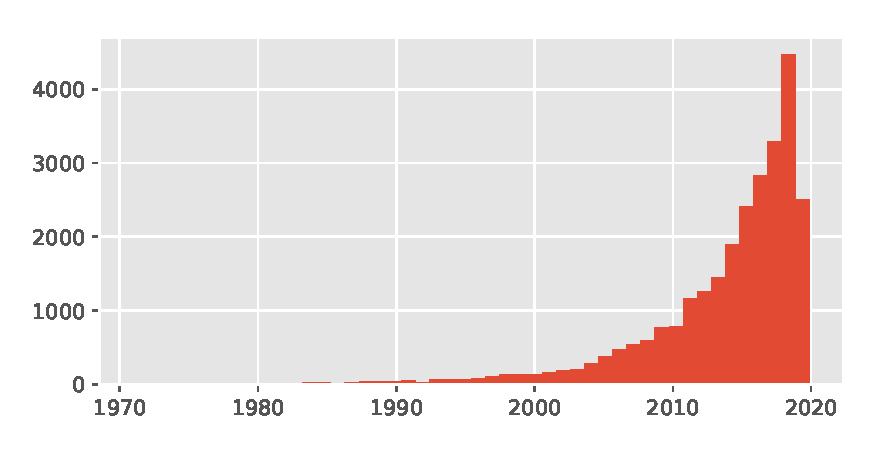
\includegraphics[width=0.8\linewidth]{images/papers_date_hist}
	\caption{Распределение статей по годам публикации.}
	\label{fig:papersdatehist}
\end{figure*}

\begin{table}
	\def\arraystretch{0.9}
	\centering
	{\small
		\begin{tabular}{lrrl}
			\toprule
			Название журнала                                    &  \# Cтатей     & \# Томов & Период     \\
			\midrule
			Neurocomputing                                      &  3187 &  334 &  1992--2019 \\
			Expert Systems with Applications                    &  2033 &  243 &  1998--2019 \\
			Procedia Computer Science                           &  1933 &  139 &  2010--2019 \\
			Pattern Recognition                                 &  1360 &  301 &  1973--2019 \\
			Applied Soft Computing                              &  1236 &  117 &  2003--2019 \\
			Information Sciences                                &  1211 &  350 &  1998--2019 \\
			Pattern Recognition Letters                         &  1001 &  292 &  1982--2019 \\
			Knowledge-Based Systems                             &  820 &  210 &  1988--2019 \\
			Journal of Systems and Software                     &  760 &  202 &  1998--2019 \\
			IFAC Proceedings Volumes                            &  743 &  280 &  1978--2014 \\
			Information and Software Technology                 &  688 &  236 &  1987--2019 \\
			Neural Networks                                     &  661 &  166 &  1989--2019 \\
			Computational Statistics \& Data Analysis            &  628 &  168 &  1988--2019 \\
			Information Processing \& Management                 &  549 &  121 &  1988--2019 \\
			Engineering Applications of Artificial Intelligence &  500 &  144 &  1992--2019 \\
			\bottomrule
	\end{tabular}}
	\caption{Статистика по 15 журналам издательств Springer и Elsevier с наибольшим количеством публикаций в коллекции.}
	\label{table:papers}
\end{table}

% ------------------------------------------------------------------------------
\subsection{Таксономия науки о данных}

Таксономия --- форма представления знаний об иерархических отношениях внутри некоторой предметной области.

Наиболее известные таксономии разработаны в рамках проекта Gene Onthology Project (GO) \cite{gene2018gene}, посвященного созданию унифицированной терминологии для аннотации генов биологических видов, и проекта SNOMED CT \cite{lee2013survey}, который представляет собой систематизированную машинно-обрабатываемую медицинскую номенклатуру, которая отражает понятия различных категорий медицины и здравоохранения

Математически таксономия представляется в виде корневого дерева --- ациклического связанного направленного графа, в котором между любыми двумя вершинами существует ровно один путь. Вершины дерева представляет собой различные понятия предметной области. Иерархические отношения отвечают отношениям включения: если вершина A --- родитель вершины B, то понятие B является частным случаем понятия A. Важной характеристикой таксономий является то, что у каждой вершины может быть только один родитель. 

Задача построения таксономий традиционно решалась вручную с помощью экспертных знаний о предметной области \cite{usman2017taxonomies}. Подобный подход имеет несколько недостатков, а именно:
\begin{itemize*}
	\item Таксономия имеет поверхностный характер и не включает в себя множество мелких и узкоспециализированных понятий и тем, которые используются в исследованиях.
	\item Наполнение таксономии происходит медленно и новые темы включаются в нее с большим запаздыванием.
	\item Экспертная оценка, как правило, не включает в себя статистический анализ предметной области и не является основанной на данных, поэтому может быть смещенной.
\end{itemize*}

Второй подход к созданию таксономий --- автоматическое их построение с помощью тематических коллекций текстов, ключевых слов и т.п. Одним из методов является трехфакторный метод Klink, впервые предложенный в \cite{Osborne2012} группой исследователей под руководством Ф. Осборна, который позволял на основе коллекции ключевых слов научных статей построить таксономию области науки. В дальнейшем на основе этого метода авторы построили полноценную систему для построения онтологий предметной области \cite{Osborne2015} и запустили на основе нее несколько веб-сервисов, позволяющих интерактивно просматривать статистические данные по существующим темам исследований \cite{Salatino2018}, а так же отслеживать изменение и зарождение новых тем \cite{Osborne2013}. Кроме того, авторами предложена система рекомендаций на основе построенной онтологии \cite{Thanapalasingam2018}. Еще один способ автоматического построения таксономий детально описан в \cite{usman2017taxonomies}.

Несмотря на то, что развитие автоматических методов создания таксономий выглядит наиболее перспективно, такой подход обладает рядом недостатков:
\begin{itemize*}
	\item Алгоритмы построения таксономий зависят от большого количества параметров и качество результата однозначно определяется оптимальностью их выбора.
	\item Тщательный подбор параметров по-прежнему требует экспертных знаний предметной области. Таким образом, человеческий фактор, присущий ручным методам построения таксономий, при применении автоматических алгоритмов не исключается.
	\item Полученные таксономии требуют ручной корректировки из-за наличия определенного количества шума: ошибочных связей, нерелевантных вершин, возможного дублирования понятий в разных вершинах.
\end{itemize*}
Более того, таксономии, созданные вручную, несмотря на их недостатки, обычно сочетают в себе как теоретические основы предметной области, так и практический опыт, накопленный людьми, участвовавшими в разработке. Именно поэтому в данной работе принято решение использовать наиболее известную таксономию компьютерных наук ACM Computing Classification System 2012 \cite{associationforcomputingmachinery}, разработанную международной Ассоциацией вычислительной техники (Association for Computing Machinery, ACM). В частности, модифицированное подмножество этой таксономии, связанное с науками о и с (машинным обучением, дата-майнингом, анализом данных, кластер-анализом и т.д.), было использовано в \cite{mirkin2018preprint}. В дополнение к исходной таксономии авторы добавили 68 новых вершин (из которых 60 --- листья), связанных с наиболее современными направлениями исследований. В модифицированной таксономии наук о данных при присутствует 456 вершин, из которых листьями являются 353 вершины. Максимальная глубина таксономии --- 6. Первые два уровня таксономии представлены в таблице \ref{table:acm_higher_ranks}. Полная версия таксономии представлена в приложении \ref{appendix:ds_taxonomy}.
.

\begin{table}[h]
	\def\arraystretch{1.}
	\centering
	\caption{Первые два уровня модифицированной таксономии наук о данных, основанной на ACM Computing Classification System 2012.}
	\label{table:acm_higher_ranks}
	\begin{tabular}{|l|l|}
		\hline
		Идентификатор & Заголовок                                             \\
		\hline
		1.             & ~~~~Theory of computation                             \\
		1.1.           & ~~~~~~~~Theory and algorithms for application domains \\
		2.             & ~~~~Mathematics of computing                          \\
		2.1.           & ~~~~~~~~Probability and statistics                    \\
		3.             & ~~~~Information systems                               \\
		3.1.           & ~~~~~~~~Data management systems                       \\
		3.2.           & ~~~~~~~~Information systems applications              \\
		3.3.           & ~~~~~~~~World Wide Web                                \\
		3.4.           & ~~~~~~~~Information retrieval                         \\
		4.             & ~~~~Human-centered computing                          \\
		4.1.           & ~~~~~~~~Visualization                                 \\
		5.             & ~~~~Computing methodologies                           \\
		5.1.           & ~~~~~~~~Artificial intelligence                       \\
		5.2.           & ~~~~~~~~Machine learning                              \\
		\hline
	\end{tabular}
\end{table}

	
% ------------------------------------------------------------------------------
\oldsubsection{Метод и вычисление матрицы релевантности текст -- словосочетание}

Наиболее популярными методами оценки релевантности тестовых документов к заданному словосочетанию (запросу) являются (а) методы, основанные на непосредственном сравнении строк, (б) основанные на сравнении некоторых термов, извлеченных из текстов (словосочетаний, $n$-грамм и т.д.) \cite{gomaa2013survey}. Кроме этого, в последние годы набирают популярность методы, учитывающие не только синтаксическую близость текстов, но и семантическую. В частности, это модели, помещающие все слова языка в некоторое векторное пространство большой размерности, где расстояние между словами характеризует их семантическую и смысловую близость. При построении векторного пространства используется как классические статистические методы \cite{Erk_2012}, так и основанные на глубинном обучении \cite{li2018word}.

В данной работе используется метод аннотированного суффиксного дерева, впервые предложенный R.Pampapathi \cite{Pampapathi_2006} в приложении к анти-спам фильтрации электронных писем. Далее метод был развит Е.Черняк и Б.Миркиным в \cite{Chernyak_2015, Chernyak_Mirkin_2015}. Преимуществами данного метода является то, что он не требует серьезной предобработки текстов (стемминга, лемматизации и. т.п.) и позволяет оценить релевантность словосочетания (короткой строки) к тексту, основываясь исключительно на данных о частотности и последовательности символов в тексте (без семантического составляющей).

Аннотированное суффиксное дерево (Annotated Suffix Tree, AST) --- это взвешенное корневое дерево, используемое для хранения фрагментов текста и их частотностей в исходном тексте. $k$-суффиксом строки $s=c_1c_2\ldots c_N$ называется фрагмент этой строки $s^k=c_{N-k+1}c_{N-k+2}\ldots c_{N}$. К примеру, 3-суффиксом строки "<information"> является строка "<ion">, а 6-суффиксом является строка "<mation">. Вершины AST отвечают следующим условиям:
\begin{itemize*}
	\item Каждая вершина соответствует одному символу строки.
	\item Каждая вершина аннотирована частотой встречи текстового фрагмента, который закодирован с помощью пути от корня дерева до этой вершины.
	\item Корень дерева не имеет символа и аннотации.
\end{itemize*}

Наивный алгоритм построения AST представлен ниже.

\begin{enumerate*}
	\item Инициализировать AST одной вершиной T (корнем дерева).
	\item Найти все суффиксы заданной строки $s$: $\{s^k=c_{N-k+1}c_{N-k+2}\ldots c_{N}, \ k=1,\ldots, N\}$.
	\item Для каждого суффикса найти максимальный путь из корня, символы вершин на котором совпадают с начальным фрагментом суффикса $s^{k_max}$, после чего аннотированное значение каждой из вершин на этом пути необходимо увеличить на единицу. Если длина пути $k_{max}$ оказывается меньше длины суффикса $k$, то к пути добавляются новые вершины, отвечающие каждому из символов оставшейся части суффикса. Аннотации новых вершин инициализируются единицей.
\end{enumerate*}
Вычислительная сложность такого алгоритма составляет $O(N^2)$. Существуют его более эффективные версии, использующие в качестве структуры данных суффиксные массивы и суффиксные деревья \cite{Grossi_2005}. Модифицированная версия алгоритма позволяет строить AST за линейное время $O(N)$.

После того, как аннотированное суффиксное дерево $T$ с корнем $R$ для текста построено, возникает задача оценки релевантности этого текста к произвольно заданной строке $x$. Авторами в \cite{MirkinChernyak2012} предложен следующий алгоритм:
\begin{enumerate*}
	
	\item  Для каждой вершины $u$ дерева $T$ вычисляется условная вероятность:
	{\sffamily
	\begin{equation}
		p(u)=\begin{cases}
			\displaystyle	\frac{f(u)}{f(\text{parent}(u))}, & \text{parent}(u) \ne R,\\[15pt]
			\displaystyle	\frac{f(u)}{\sum_{v\in T:\ \text{parent}(v)=R}f(v)}, & \text{parent}(u) = R,
		\end{cases}
	\end{equation}
	}
	где $f(u)$ --- аннотация вершины $u$. 
	\item Для каждого $k$-суффикса строки $x$ вычисляется коэффициент его релевантности тексту, хранимому в дереве $T$. 
	\begin{equation}
		s(x^k, T)=\frac{1}{k_{max}}\sum_{i=1}^{k_{max}}p(x_i^k),
	\end{equation}
	\item Релевантность строки $x$ тексту, хранимому в $T$, вычисляется как среднее значение коэффициентов релевантности всех суффиксов строки:
	\begin{equation}
		S(x,T)=\frac1N\sum_{k=1}^{N}s(x^k, T).
	\end{equation}
\end{enumerate*}

На практике вместо построения одного большого аннотированного суффиксного дерева для целого текста, текст разбивают на набор коротких строк, состоящих из 2-5 последовательно идущих слов, после чего по очереди добавляют каждую из строк в AST с помощью алгоритма, описанного выше.

Перед построением AST тексты предобрабатываются следующим образом:
\begin{enumerate*}
	\item Символы текста приводятся к нижнему регистру.
	\item Удаляется пунктуация (символы, не являющиеся пробельными символами, буквами или цифрами).
	\item Для того, чтобы уменьшить влияние наиболее часто встречающихся слов, удаляются стоп-слова\footnote{\hrefl{https://raw.githubusercontent.com/nltk/nltk\_data/gh-pages/packages/corpora/stopwords.zip}}.
	\item Текст разрезается на множество фрагментов по 5 слов.
\end{enumerate*}

После построения AST временная сложность получения оценки релевантности строки к тексту составляет $O(m^2)$, где $m$ --- длина оцениваемой строки.

Таким образом, для получения матрицы релевантности статей к листьям таксономии, необходимо для каждой из аннотаций статей построить AST, после чего для каждого из словосочетаний, привязанных к листьям таксономии, получить оценку его релевантности. Для набора данных, описанного в \ref{section:text-data}, итогом работы алгоритма является матрица действительных чисел $T=(t_{ij})$ размера $26799 \times 353$.

%%% пример работы?

% ------------------------------------------------------------------------------
\subsection{Метод построения таблицы корелевантности словосочетаний}

Схожесть тем (словосочетаний) $i$ и $j$ может быть определена как скалярное произведение векторов $t_i=(t_{vi})$ и $t_j=(t_{vj})$, ($v=1,\ldots,26799$), где каждый текст взвешен коэффициентом, отражающим количество тем, релевантных этому тексту. Такая поправка необходима, чтобы придать документам с большим количеством релевантных тем больший вес в скалярном произведении (см. \cite{mirkin2010constructing}). Веса определяются следующим образом:

\begin{equation}
		w_{v} = \frac{n_v}{\max_{v'} n_{v'}}, \quad n_v = \#_i[t_{vi} > \alpha]
	\label{eq:rel_wt}
\end{equation}
где $\alpha$ --- порог, определяемый эмпирически (см. \cite{Chernyak_2015}). Для соответствия распределения количества релевантных вершин $n_v$ источнику \cite{mirkin2018preprint}, выбрано значение $\alpha=0.4$. Это распределение $n_v$ приведено в таблице и на рисунке \ref{fig:relevant_counts}.

C учетом вышесказанного, таблица корелевантности тем определяется следующим образом:
\begin{equation}
	R = (r_{ij}), \   r_{ij} = \sum_{v} w_{v} t_{vi} t_{vj}, \ \ i,j\in[1,\ldots, 353].
	\label{eq:rel}
\end{equation}

\begin{figure}[b]
	\centering
	\caption{Распределение релевантных тем в текстовой коллекции.}
	\label{fig:relevant_counts}
	\begin{minipage}{0.45\textwidth}
		\centering
		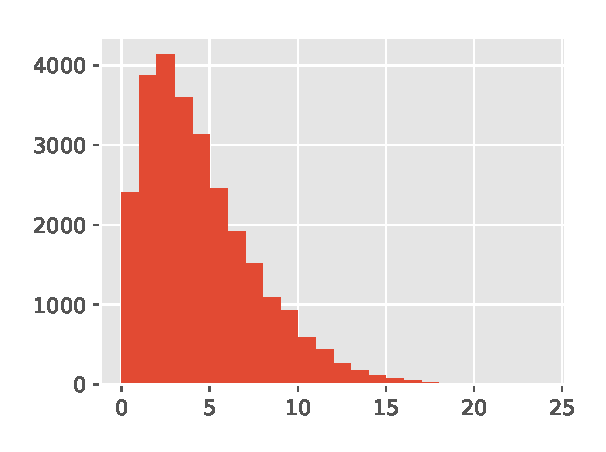
\includegraphics[width=0.9\textwidth]{images/relevants_hist}
	\end{minipage}
	\begin{minipage}{0.45\textwidth}
		\centering
		\begin{tabular}{|p{0.45\textwidth}|p{0.45\textwidth}|}
			\hline 
			Количество текстов & Количество релевантных тем \\ 
			\hline 
			2401 (9\%)  & 0 \\ 
			3867 (14\%)   & 1 \\ 
			10868 (41\%)  & 2-4 \\ 
			8921 (33\%)   & 5-11 \\ 
			742 (3\%)    & 12 и более \\ 
			\hline 
		\end{tabular} 
	\end{minipage}
\end{figure}

Известно (см. \cite{MirkinChernyak2012}), что матрица $R$, определенная уравнениями \eqref{eq:rel} и \eqref{eq:rel_wt}, обладает следующими свойствами:

\begin{itemize*}
	\item $R$ неотрицательно определена.
	\item $r_{ij}>0$ в том случае, если существует хотя бы один текст, к которому релевантны сразу обе темы $i$ и $j$.
	\item Чем больше количество текстов, релевантных темам $i$ и $j$, тем больше значение $r_{ij}$.
\end{itemize*}

% ------------------------------------------------------------------------------
\subsection{Метод и кластер-анализ таблицы корелевантности}

Обозначим множество листовых вершин с соответствующими им темами $T$. Нечеткий кластер над $T$ определяется функцией принадлежности $u=(u_t)$, ($u_t\in[0,1], t\in T$) и коэффициентом интенсивности $\mu>0$, который связывает значения функции принадлежности с значениями функции схожести. В случае, когда $T$ --- набор тем академических исследований, $u=(u_t),\ t\in T$ --- кластеры, характеризующие семантическую структуру коллекции текстов, произведение $(\mu u_t)(\mu u_{t'}) = \mu^2u_tu_{t'}$ может рассматриваться как вклад направления исследований, определяемого кластером, в коэффициент корелевантности $r_{tt'}$ между темами $t$ и $t'$. Это предположение согласуется с моделью аддитивной нечеткой кластеризации, предложенной С. Насименто и Б. Миркиным в \cite{mirkin2009analysis}. Утверждается, что элементы матрицы корелевантности тем $R$ могут быть представлены как сумма вкладов $K$ нечетких кластеров, а именно:
\begin{equation}
	r_{tt'}=\sum_{k=1}^{K}\mu_k^2u_{kt}u_{kt'} + \epsilon_{tt'},
	\label{eq:faddis_crit}
\end{equation}
где $\epsilon_{ij}$ --- малые ошибки, $u_k=(u_{kt})$ --- вектор значений функции принадлежности $k$-го кластера , $\mu_k$ --- его интенсивность. 

Метод FADDIS, разработанный в \cite{mirkin2009analysis, mirkin2012additive, nascimento2013laplacian}, позволяет с помощью итеративной процедуры извлекать из матрицы схожести нечеткие кластеры согласно критерию \eqref{eq:faddis_crit}. Авторами проведены численные эксперименты, показывающие корректность метода на реальных и синтетических наборах данных.

На каждом шаге работы алгоритма FADDIS рассматривается задача минимизации критерия наименьших квадратов для одного кластера:

\begin{equation}
	E=\sum_{t,t'\in T}(w_{tt'}-\xi u_t u_{t'})^2,
	\label{eq:faddis_onestep_crit}
\end{equation}
где $W=(w_{tt'})$ --- матрица сходства элементов $t\in T$, а неизвестными параметрами являются $\xi>0$ --- вес кластера и $u=(u_t)$ --- вектор принадлежности элементов $t\in T$ кластеру. Значение интенсивности из \eqref{eq:faddis_crit} определяется как $\mu=\sqrt{\xi}$.

На первом шаге алгоритма в качестве $W$ берется исходная матрица сходства $R$. На втором и последующих шагах $W$ определяется как остаток от вычитания из матрицы сходства на предыдущем шаге вклада кластера, найденного с помощью оптимизации критерия \eqref{eq:faddis_onestep_crit}:

\begin{equation}
	W  \gets W - \mu^2uu^T.
\end{equation}

Каждый элемент матрицы $R$, таким образом, действительно представляет собой сумму вкладов индивидуальных кластеров с точностью до малых ошибок. Количество кластеров $K$ может быть определено как заранее, так и в процессе работы алгоритма согласно некоторому критерию остановки.

Для минимизации целевой функции \eqref{eq:faddis_onestep_crit} относительно $\xi$ при заданном произвольном векторе $u$ продифференцируем ее по $\xi$ и получим необходимое условия существования ее экстремума:

\begin{equation}
	\frac{\partial E}{\partial \xi}= -2\sum_{t,t'\in T}(w_{tt'}-\xi u_t u_{t'}) u_t u_{t'} =0.
\end{equation}
Из этого уравнения получим выражение для оптимального $\xi$:

\begin{equation}
	\xi = \frac{\sum_{t,t'\in T}w_{tt'} u_t u_{t'}}{(\sum_{t \in T}u_t^2)^2},
\end{equation}
В матричном виде:

\begin{equation}
\xi = \frac{u^TWu}{(u^Tu)^2},
\end{equation}
В случае, когда матрица $W$ неотрицательно определена, значение $\xi$ всегда неотрицательно. Подставляя $\xi$ в \eqref{eq:faddis_onestep_crit}, получим:

\begin{equation}
	E = \sum_{t,t'\in T}w_{tt'}^2-\xi^2 \sum_{t\in T}u_t^2 \sum_{t'\in T}u_{t'}^2 = S(W) - G(u),
\end{equation}
где $S(W)=\sum_{t,t'\in T}w_{tt'}^2$ --- разброс данных, $G(u) = \xi^2 (u^Tu)^2= \left(\frac{u^TWu}{u^Tu}\right)^2$. Таким образом, разброс данных может быть представлен в виде суммы объясненной и необъясненной кластером $u$ частей:
\begin{equation}
	S(W)=G(u)+E.
\end{equation}
И, так как $S(W)$ зависит только от исходной матрицы $W$ и является константой по отношению к $u$, задача минимизации $E$ эквивалентна задаче максимизации $G(u)$ или квадратного корня из этой величины:
\begin{equation}
	g(u)=\sqrt{G(u)} = \frac{u^TWu}{u^Tu}.
	\label{eq:rayleigh}
\end{equation}
Величина  $g(u)$ называется отношением Релэя \cite{parlett1998symmetric}. Для случая безусловной оптимизации известно, что максимум этого отношения равен максимальному собственному значению матрицы $W$ и достигается на соответствующем собственном векторе $z$. Для получения субоптимального решения задачи условной оптимизации с ограничением $u_t\in[0, 1], t\in T$ воспользуемся следующим методом:
\begin{enumerate*}
	\item Получим решение безусловной задачи оптимизации в виде нормализованного собственного вектора $z:\ z^Tz=1$, отвечающего максимальному собственному значению матрицы $W$.
	\item Воспользуемся оператором проекции на множество векторов ${v:\ \forall t\in T\ v_t\in[0, 1]}$:
	\begin{equation}
		v_t =\begin{cases}
		0, & z_t \leq 0,\\
		z_t, & 0<z_t<1\\
		1, & z_t\geq 1.
		\end{cases}
	\end{equation}
	Нужно заметить, что исходный вектор $z$ нормирован и поэтому третье условие не выполнится никогда. Несмотря на это, оставим его для большей наглядности.
	\item В выражениях для $\xi, g(u)$ присутствует величина $u^Tu$, поэтому естественным методом нормировки будет $u^Tu=\sum_{t\in T} u_t^2=1$. Нормируем полученный на предыдущем шаге вектор:
	\begin{equation}
		u = \frac{v}{\sqrt{v^Tv}}.
	\end{equation}
\end{enumerate*}

Полученному вектору $u$ отвечает значение веса кластера $\xi=u^TWu$ и значение вклада в разброс данных $G(u)=(u^TWu)^2=\xi^2$. Необходимо заметить, что, так как вектор ($-z$) тоже является собственным вектором, отвечающим максимальному собственному значению матрицы $W$, использование в шаге 2 значения $-z_t$ вместо $z_t$ так же ведет к получению корректного вектора $u$. В этом случае в качестве решения следует взять вектор, соответствующий более высокому значению вклада $G(u)$ кластера в разброс данных $G(u)$.

Процесс итеративного извлечения кластера останавливается, когда выполняется одно из следующих условий:
\begin{enumerate*}
	\item\label{enum:faddis_stop_xi_neg} Значение $\xi$, полученное на текущем шаге, отрицательное.
	\item Вклад извлеченного на данном шаге кластера меньше некоторого порога. К примеру, вклад должен быть больше среднего вклада одного объекта.
	\item Остаточный разброс данных $E$ становится меньше, к примеру, 5\% от начального значения разброса.
	\item Достигнуто заданное заранее количество кластеров.
\end{enumerate*}

Для того, чтобы сделать структуру кластеров в начальных данных более явной, применяется дискретное нормализованное преобразование Лапласа \cite{von2007tutorial}. Подобное преобразование используется при нахождении субоптимального решения для задачи наименьшего нормализованного разреза (min normalized cut). Известно, что решением этой задачи является собственный вектор, отвечающий наименьшему ненулевому собственному значению преобразованной матрицы смежности графа. Алгоритм FADDIS, в свою очередь, требует нахождения \emph{наибольшего} собственного значения и отвечающего ему собственного вектора. Именно поэтому в \cite{mirkin2012additive} предложено использовать модифицированое преобразование Лапласа, задействующее обратные собственные значения матрицы смежности. 

Нормализованное преобразование Лапласа для матрицы $W$ определяется следующим образом:
\begin{equation}
	L_n=I-D^{-\frac{1}{2}}WD^{-\frac{1}{2}}, 
\end{equation}
где $I$ --- единичная матрица аналогичного $W$ размера, $D$ --- диагональная матрица, в которой $d_{tt} =\sum_{t'\in T} w_{tt'}$. 
Тогда псевдо-обратным преобразованием Лапласа (Laplacian pseudo-inverse transform, LAPIN) \cite{nascimento2013laplacian} называется следующая матрица:
\begin{equation}
	L_n^+ = Z \tilde{\Lambda}^{-1} Z^T,
\end{equation}
где $Z$ --- матрица собственных векторов, отвечающих ненулевым собственным значениям матрицы $L_n$ (из ее спектрального разложения $L_n=Z\Lambda Z^T$), $\tilde{\Lambda}$ --- матрица, получаемая из матрицы $\Lambda$ удалением нулевых значений на диагонали.

Для решения задачи кластеризации с помощью FADDIS исходная матрица схожести $R$ преобразовывается с помощью LAPIN, после чего применяется описанный выше алгоритм построения нечетких кластеров.

% ------------------------------------------------------------------------------
\subsection{Программное обеспечение}

В результате работы над дипломным проектом был разработан комплекс программ. Разработка велась на языке Python версии 3.6.8. Коды программ доступны в репозитории автора на GitHub\footnote{\hrefl{https://github.com/alvlasov/master-thesis}}.

Расчеты проводились на личном ноутбуке с процессором Intel Core-i5 и 8 ГБ RAM, а так же на доступных автору вычислительным мощностям (сервер DELL R640).

\subsubsection{Подготовка данных}

\begin{itemize*}
	
	\item Для подготовки "<сырых"> данных текстовой коллекции, выгруженных из электронной библиотеки, разработано программное обеспечение со следующими функциями:
	\texttt{}
	\begin{enumerate*}
		\item Извлечение из текста названия журнала, номера тома и даты публикации из необработанных текстовых данных (см. приложение \ref{appendix:raw_text_sample}).  
		\item Очистка коллекции от нерелевантных журналов, журналов с некорректно распознанными датами и т.п.
		\item Предобработка текстов согласно разделу \ref{section:text-data}.
	\end{enumerate*}
	
	
	\item Портирована с языка Python 2 на Python 3 библиотека \texttt{EAST}, реализующая эффективные методы построения аннотированного суффиксного дерева и оценки релевантности строк с его помощью. Адаптированная версия доступна в репозитории автора на GitHub\footnote{\hrefl{https://github.com/alvlasov/AST-text-analysis}}.
	\item Разработаны скрипты для параллельного построения AST и оценки релеватности для большой коллекции документов.
	\item Разработан скрипт для предобработки используемой таксономии (использована библиотека \texttt{anytree}\footnote{\hrefl{https://github.com/c0fec0de/anytree}}).
	\item Разработаны программы для построения матрицы релевантности документа к темам и матрицы корелевантности тем.
	\item Программно реализован метод преобразования матриц LAPIN.
\end{itemize*}



\subsubsection{Формирование кластеров}
Реализован программно метод нечеткой кластеризации FADDIS\footnote{\hrefl{https://github.com/alvlasov/cluster-analysis}}.
%%%% еще?

\subsubsection{Обобщение кластеров}
Реализованы программно:
\begin{itemize*}
	\item Алгоритм экономичного обобщения ParGenFS с функцией накопления статистики потерь/приобретений по вершинам для последующего использования критерия максимального правдоподобия.
	\item Алгоритм максимально правдоподобного обобщения MaLGenFS.
\end{itemize*}

%%%% еще?
\subsubsection{Графика и визуализация}
Реализованы программно:

\begin{itemize*}
	\item Скрипт для автоматической визуализации таксономии с нанесением на нее информацией об обобщаемом кластере, его головными понятиями, пропусками и выбросами. Использована библиотека \texttt{ETE Toolkit}\footnote{\hrefl{http://etetoolkit.org/}}.
	\item Скрипт для построения диаграммы пересечений обобщенных кластеров.	
\end{itemize*}

%%%% еще?
% ------------------------------------------------------------------------------
\subsection{Результаты расчетов и выводы}

В ходе численного эксперимента сделано следующее:

\begin{enumerate*}
	\item\label{enum:experiment_log_start} Подготовлена коллекция аннотаций научных статей, ее размер --- 26799 текстов.
	\item Подготовлена таксономия "<Наук о данных">.
	\item С помощью AST сформирована матрица релевантности текстов к темам, соответствующим листовым кластерам таксономии. Размер матрицы: $26799 \times 353$.
	\item Матрица релевантности преобразована в квадратную матрицу корелевантности тем размера  $353\times 353$.
	\item\label{enum:experiment_log_faddis} С помощью метода FADDIS получено 35 нечетких кластеров на множестве тем. В качестве критерия остановки использовано условия положительности веса кластера $\xi$. 
	\item Для исключения шумовых элементов из кластеров удалены те темы, функция принадлежности которых меньше 0.1.
	\item\label{enum:experiment_log_pars} Полученные кластеры обобщены с помощью ParGenFS. Наиболее репрезентативные из них представлены на рисунках \ref{fig:tax_learning}-\ref{fig:tax_structuring}.
	\item Применен метод MaLGenFS:
	\begin{alphaenumerate*}
		\item На случайных подвыборках исходной коллекции статей выполнены пункты \ref{enum:experiment_log_start}-\ref{enum:experiment_log_pars}. Размер подвыборок --- 20\% от коллекции.
		\item Полученное множество нечетких кластеров дефаззифицировано на уровне 0.1.
		\item Построены обобщения каждого из кластеров, накоплена статистика по потерям и приобретениям в вершинах, вычислены вероятности событий.
		\item Кластеры, использованные в \ref{enum:experiment_log_pars}, дефаззифицированы на уровне 0.1 и повторно обобщены с использованием MaLGenFS.
	\end{alphaenumerate*}
\end{enumerate*}

\subsubsection{Обобщение кластеров с помощью критерия наибольшей экономии}

В пункте \ref{enum:experiment_log_faddis} эксперимента получено 35 кластеров, из которых:
\begin{itemize*}
	\item 15 кластеров не получили ни одного головного понятия. Элементы этих кластеров очень слабо связаны между собой. Одним из объяснений их появления является наличие некоторого количества шума в исходной коллекции текстов, а так же использование метода AST, который учитывает исключительно синтаксическую схожесть текстов (к примеру, оценка схожести AST слов "<morphology"> и "<onthology"> высока, несмотря на то что эти термины принадлежат совершенно разным областям наук о данных).
	\item 7 кластеров имеют меньше 10 листовых элементов. Эти кластеры, в основном, имеют одно или два головных понятия и несколько выбросов со значением функций принадлежности $u<0.4$. Такие кластеры не представляют большого интереса, т.к. объединяют слишком малое множество вершин таксономии.
	\item 7 кластеров являются легко интерпретируемыми. 
\end{itemize*}

Наиболее репрезентативные и интерпретируемые обобщения кластеров приведены на рисунках \ref{fig:tax_learning}-\ref{fig:tax_structuring}. В таблице \ref{table:pars_results} представлена подробная информация по этим кластерам.

В \cite{mirkin2018preprint} были получены обобщения трех интерпретируемых кластеров: "<Learning">, "<Retrieval">, "<Clustering">.
Головные понятия и один выброс обоих кластеров "<Learning"> в точности совпадают, что подтверждает корректность расчетов в данной работе.
Обобщение кластера "<Clustering"> в данной работе получилось более плотным: в нем всего 9 элементов (в \cite{mirkin2018preprint} получилось 16 элементов).
Кластер "<Retrieval"> значительно отличается между двумя работами. В \cite{mirkin2018preprint} этот кластер содержит в себе головное понятие "<Computer Vision">, которое в данной работе принадлежит кластеру "<Structuring">. Остальные кластеры являются уникальными для данной работы.

\newcommand{\offshoot}{$\bigodot \ $}
\newcommand{\gap}{$\bigotimes\ \ $}
\newcommand{\makecelll}[1]{\makecell[l]{#1}}
\begin{center}
	\def\arraystretch{0.7}
	{\footnotesize \begin{longtable}{|l|l|l|c|c|}
			\caption{Наиболее репрезентативные обобщения кластеров, полученные с помощью алгоритма ParGenFS. Приведены элементы с функцией принадлежности $u>0.15$. Символом \offshoot обозначены выбросы.}
			\label{table:pars_results}\\
			\hline
			Интерпретация  & Головные понятия и выбросы & \makecelll{Кол-во\\пропусков} & \makecelll{Кол-во листьев \\в кластере} \\ 
			\hline
			\endhead
			\hline
			\multicolumn{4}{r}{{Продолжение на след. странице}} \\
			\endfoot
			\hline
			\endlastfoot
		\makecelll{"<Обучение">\\("<Learning">)} & \makecelll{1.1.1. -- Machine learning theory\\
		5.2. -- Machine learning\\
		\offshoot 3.4.4.5. -- Learning to rank}
	& 38 & 32
		   \\ 
		\hline 
		\makecelll{"<Кластеризация">\\("<Clustering">)} & \makecelll{3.2.1.4. -- Clustering\\
		\offshoot	1.1.1.3. -- Unsupervised learning and clustering\\
		\offshoot	2.1.5.8. -- Cluster analysis\\
		\offshoot	3.2.1.7.3 -- Graph based conceptual clustering\\
		\offshoot	3.2.1.9.2. -- Trajectory clustering\\
		\offshoot	3.4.5.8. -- Clustering and classification\\
		\offshoot	5.2.1.2.1. -- Cluster analysis\\
		\offshoot	5.2.3.2.5 -- Kernel-based clustering\\
		\offshoot	5.2.4.3.1 -- Spectral clustering\\
		} & 0 & 17\\ 
		\hline 
		\makecelll{"<Вероятностные\\представления">\\("<Probabilistic\\representations">)}   & \makecelll{2.1.1. -- Probabilistic representations\\
			5.2.1.2. -- Unsupervised learning\\
			5.2.3.5. -- Learning in probabilistic graphical models\\
			\offshoot 1.1.1.4.3. -- Modelling\\
			\offshoot 1.1.1.6. -- Bayesian analysis\\
			\offshoot 3.1.1.3.2. -- Network data models\\
			\offshoot 3.3.1.4. -- Web log analysis\\
			\offshoot 3.4.3.2. -- Task models\\
			\offshoot 5.2.3.1.3 -- Model trees\\
			\offshoot 5.2.3.13.1. -- Deep belief networks\\
			\offshoot 5.2.3.7.2. -- Factor analysis\\
		} & 11 & 31\\ 
		\hline 
		\makecelll{"<Извлечение">\\("<Retrieval">)}& \makecelll{3.1.4. -- Query languages\\
			3.4. -- Information retrieval\\
			\offshoot  5.1.1.9. -- Language resources
		} & 27 & 28\\ 
		\hline 
		\makecelll{"<Структуризация">\\("<Structuring">)}  & \makecelll{3.1.1.5. -- Data model extensions\\
			5.1.3. -- Computer vision\\
			\offshoot 1.1.1.12. -- Structured prediction\\
			\offshoot 1.1.2.10. -- Logic and databases\\
		\offshoot 	3.1.2.1.2. -- Data scans\\
			\offshoot 3.1.3.3.3. -- Database recovery\\
		\offshoot 	3.1.3.7. -- Database views\\
		\offshoot 	3.1.4.1.1. -- Structured Query Language\\
		\offshoot 	3.1.5.9. -- Federated databases\\
		\offshoot 	3.2.1.4.5 -- Feature weight clustering\\
		\offshoot 	3.4.1.1. -- Document structure\\
		\offshoot 	3.4.2.1. -- Query representation\\
		\offshoot 	3.4.4.8. -- Top-k retrieval in databases\\
		\offshoot 	3.4.7.1.1. -- Structured text search\\
		\offshoot 	5.1.1.6. -- Speech recognition\\
		\offshoot 	5.2.1.1.5. -- Structured outputs\\
		\offshoot 	5.2.3.3.3.2 -- Fuzzy representation\\
		\offshoot 	5.2.3.6.2.1 -- Tensor representation\\
		\offshoot 	5.2.3.7.3.1 -- 2D PCA\\
		}  & 11   & 34\\ 
		\hline 
		\makecelll{"<Представления в\\компьютерном зрении">\\("<Computer vision\\representations">)} &  \makecelll{5.1.3.2. -- Computer vision representations\\
			\offshoot 	4.1.4.1. -- Visualization toolkits\\
			\offshoot 	5.2.3.3.3.2 -- Fuzzy representation\\
			\offshoot 	5.2.3.6.2.1 -- Tensor representation\\
			\offshoot 	5.2.3.7.3.1 -- 2D PCA\\
		} &0 & 13\\ 
		\hline 
		\makecelll{"<Запросы">\\("<Querying">)}  & \makecelll{3.1.3.2. -- Database query processing\\
			3.4.2. -- Information retrieval query processing\\
			\offshoot 2.1.5.1. -- Queueing theory\\
			\offshoot 3.1.4.2.2. -- XQuery\\
			\offshoot 4.1.2.5. -- Dendrograms\\
			\offshoot 5.1.2.5. -- Vagueness and fuzzy logic\\
			\offshoot 5.2.3.2.1.1 -- Dynamic
		}  &3 & 15 \\ 
		\hline 
	\end{longtable} }
\end{center}



\begin{figure}
	\centering
	\vspace{-2cm}
	\includegraphics[width=\textheight, angle=90, origin=c, clip]{images/cluster_lift_tree_00_learning}
	\caption{Результаты обобщения кластера "<Learning">.}
	\label{fig:tax_learning}
\end{figure}


\begin{figure}
	\centering
	\vspace{-2cm}
	\includegraphics[width=\textheight, angle=90, origin=c, clip]{images/cluster_lift_tree_01_clustering}
	\caption{Результаты обобщения кластера "<Clustering">.}
	\label{fig:tax_clustering}
\end{figure}

\begin{figure}
	\centering
	\vspace{-2cm}
	\includegraphics[width=\textheight, angle=90, origin=c, clip]{images/cluster_lift_tree_02_prob_representations}
	\caption{Результаты обобщения кластера "<Probabilistic representations">.}
	\label{fig:tax_prob_representations}
\end{figure}

\begin{figure}
	\centering
	\vspace{-2cm}
	\includegraphics[width=\textheight, angle=90, origin=c, clip]{images/cluster_lift_tree_04_retrieval}
	\caption{Результаты обобщения кластера "<Retrieval">.}
	\label{fig:tax_retrieval}
\end{figure}

\begin{figure}
	\centering
	\vspace{-2cm}
	\includegraphics[width=\textheight, angle=90, origin=c, clip]{images/cluster_lift_tree_06_structuring}
	\caption{Результаты обобщения кластера "<Structuring">.}
	\label{fig:tax_structuring}
\end{figure}

\begin{figure}
	\centering
	\vspace{-2cm}
	\includegraphics[width=0.8\textheight, angle=90, origin=c, clip]{images/cluster_lift_tree_11_cv_representations}
	\caption{Результаты обобщения кластера "<Computer vision representations">.}
	\label{fig:tax_cv_representations}
\end{figure}
\begin{figure}
	\centering
	\vspace{-2cm}
	\includegraphics[width=\textheight, angle=90, origin=c, clip]{images/cluster_lift_tree_20_querying}
	\caption{Результаты обобщения кластера "<Querying">.}
	\label{fig:tax_querying}
\end{figure}

\clearpage
\subsubsection{Обобщение кластеров с помощью критерия максимального правдоподобия}

Накопив статистику и применив алоритм MaLGenFS к дефаззифицированным кластерам из пункта \ref{enum:experiment_log_faddis} эксперимента, получили их обобщения, основанными на критерии максимального правдоподобия. Сравнивая их с обобщениями, полученными исходя из критерия наибольшей экономии, можно заключить, что метод максимального правдоподобия имеет тенденцию к сокращению числа головных понятий, и только в редких случаях добавляет новые или заменяет текущие понятия. Отличия результатов работы двух методов для 7 наиболее репрезентативных кластеров из предыдущего раздела приведены в таблице \ref{table:mals_vs_pars}. 

\begin{center}
	\centering
	{ \begin{longtable}{|c|c|}
		\caption{Сравнение результата работы алгоритма MaLGenFS с алгоритмом ParGenFS на семи наиболее репрезентативных кластерах.} \label{table:mals_vs_pars}\\
		\hline
		Кластер & Отличия MaLGenFS от ParGenFS \\
		\hline
		\endhead
		\hline
		\multicolumn{2}{r}{{Продолжение на след. странице}} \\
		\endfoot
		\hline
		\endlastfoot

			\makecell{"<Обучение">\\("<Learning">)}& Идентичны  \\ 
			\hline 
			\makecell{"<Кластеризация">\\("<Clustering">} & Идентичны \\ 
			\hline 
			\makecell{"<Вероятностные\\представления">\\("<Probabilistic\\representations">)}  & 
			
			\makecelll{
				Пропало головное понятие:\\
				5.2.1.2. -- Unsupervised learning \vspace{0.2cm}\\
				Появились новые выбросы:\\
				\offshoot 5.2.1.2.1. -- Cluster analysis\\
				\offshoot5.2.1.2.3. -- Mixture modeling\\
				\offshoot5.2.1.2.4. -- Topic modeling\\
			}  \\ 
			\hline 
			\makecell{"<Извлечение">\\("<Retrieval">)}& 	
			\makecelll{
				Пропало головное понятие:\\
				3.1.4. -- Query languages \vspace{0.2cm}\\
				Появились новые выбросы:\\
				\offshoot3.1.4.1.1. -- Structured Query Language\\
				\offshoot3.1.4.2.2. -- XQuery\\
				\offshoot3.1.4.3.1. -- MapReduce languages\\
				\offshoot3.4.1.1. -- Document structure\\
				\offshoot3.4.1.2. -- Document topic models\\
				\offshoot 3.3.4.2.2. -- Query intent\\
				\offshoot 3.5.1.1.9. -- Language resources
			} \\ 
			\hline 
			\makecell{"<Структуризация">\\("<Structuring">)}&	
			\makecelll{
				Пропали все исходные головные понятия:\\
				3.1.1.5. -- Data model extensions\\
				5.1.3. -- Computer vision \vspace{0.2cm}\\
				Появилось одно новое:\\
				5.1.3.2. -- Computer vision representations\\
			}  \\ 
			\hline 
			\makecell{"<Представления в\\компьютерном зрении">\\("<Computer vision\\representations">)}&  Идентичны \\ 
			\hline 
			\makecell{"<Запросы">\\("<Querying">)}&
			\makecelll{
				Пропало головное понятие:\\
				3.4.2. -- Information retrieval query processing \vspace{0.2cm}\\
				Появились новые выбросы:\\
				\offshoot 3.4.2.2. -- Query intent\\
				\offshoot3.4.2.3. -- Query log analysis\\
				\offshoot3.4.2.4. -- Query suggestion\\
			}  \\ 
			\hline 
	\end{longtable} }
\end{center}

Интересным фактом является то, что, несмотря на то, что обобщение было произведено на \emph{жестких} кластерах (не на нечетких, как в предыдущем разделе), результаты практически полностью совпали. Следовательно, информация о нечеткости кластеров полностью сохраняется в априорных вероятностях событий. Этот факт указывает на то, что обобщение произвольного множества с помощью метода максимального правдоподобия можно построить даже в том случае, когда исследователь не обладает достаточной экспертизой, чтобы определить значения принадлежности. Таким образом, подтверждается эффективность этого метода и превосходство его в этом аспекте над предыдущим.

\subsubsection{Исследование пересечений между кластерами}

Кластеры, которые имеют одно или больше головных понятий и некоторое количество выбросов, оказались тесно связанными в том смысле, что они имеют пересечения множества выбросов и множества головных понятий. Визуализация этого представлена на рисунке \ref{fig:clusters_interaction}. Можно видеть, что существуют две группы кластеров с тесными внутренними связями:
\begin{itemize*}
	\item Извлечение и хранение данных (выделены желтым).
	\item Визуализация данных (выделены синим).
\end{itemize*}
Эти группы связаны друг с другом через три кластера, связанные с языками для извлечения информации из хранили (выделены зеленым цветом). Особняком стоит кластер, связанный с задачами обучения без учителя (выделен фиолетовым цветом).

Полученная визуализация хорошо согласуется с общими представлениями о структуре наук о данных. Существует тесно связанный набор технологий, используемый для сбора и хранения необработанных данных. Далее, с помощью специализированных языков проводится обработка и агрегация данных. На основе обработанных данных строятся визуализации, которые являются наиболее простым и наглядным способом представления статистик, зависимостей и паттернов в данных. Кроме этого, обработанные данные могут использоваться для обучения без учителя и, в частности, для кластер-анализа, построения оценок плотности распределения данных и определения скрытых факторов, порождающих эти данные. Учитывая то, что количество неразмеченных данных с каждым днем неуклонно растет, можно заключить, что исследователи учитывают этот факт и в публикациях на тему извлечения и хранения неразмеченных больших данных зачастую поднимается тема их обработки.


\begin{figure}[h]
	\centering
	\includegraphics[width=0.8\linewidth, clip]{images/clusters_interaction}
	\caption{Диаграмма пересечения головных тем и выбросов полученных обобщений. На элементах указаны головные темы соответствующих кластеров. Цветом выделены группы кластеров, схожие по тематике: зеленым --- языки для извлечения информации из хранилищ, желтым --- хранение и извлечение информации, синим --- визуализация, фиолетовым --- задачи обучения без учителя.}
	\label{fig:clusters_interaction}
\end{figure}


\subsubsection{Тенденции развития науки о данных}

Найденные тематические кластеры показывают области наук о данных, которые часто исследуются в рамках одной и той же публикации, и могут свидетельствовать о зарождении новой области исследований, находящейся на границе каждого из элементов кластера. Если же кластер расположен плотно (у мего малое количество головных тем и выбросов), то он соответствует уже устоявшейся области исследований, которая хорошо отражена в использованной таксономии. Интерпретируя кластеры таким образом, можно заключить:

\begin{alphaenumerate*}
	\item Кластер "<Learning"> соответствует уже устоявшейся теме исследований --- методам обучения с учителем в задачах классификации, регрессии и ранжирования.
	\item  "<Сlustering"> отвечает одной из задач обучения без учителя --- кластеризации. Наличие выбросов свидетельствует о том, что несмотря на то, что методы кластер-анализа используются в различных областях, кластеризация пока что не является отдельной единой областью наук о данных (возможно, скоро придет время выделить ее в отдельную вершину более высокого уровня). 
	\item "<Probabilistic representations"> состоит из статистических методов представления данных (в том числе направленным графическим моделям и байесовским методам в статистике) и задач обучения без учителя. Это свидетельствует о том, что задачи обучения без учителя, постановка которых зачастую является эвристикой, постепенно получают математические обоснования и происходит соединение экспериментальной науки и теоретической.
	\item Кластеры "<Retrieval"> и "<Querying"> соответствуют устоявшимся областям: извлечению данных и их обработке и агрегации.
	\item Кластер "<Computer vision representations"> так соответствует устоявшейся теме исследований. Но, можно заметить, что в выбросах этого кластера находятся вершины, отвечающие техникам нечетких и тензорных представлений данных.
	\item Кластер "<Structuring"> отвечает сразу нескольким обширным темам: компьютерному зрению, теории баз данных, методам хранения данных и различным представлениям данных. В том числе в выбросах присутствует темы, связанные с распознаванием речи и поиску в текстах. Все  эти темы объединяет то, что объектом исследованиний в них являются различные методы работы с \emph{неструктурированными} данными сложной структуры, для автоматического извлечения информации из которых требуются серьезные усилия и сложные алгоритмы. Можно надеяться на то, что в ближайшее время возникнет новая область исследований, в рамках которой будут разработаны общие подходы к решению проблемы обработки неструктурированных данных, которые будут использовать независимо от того, какого рода данные обрабатываются. 
\end{alphaenumerate*}


% ==============================================================================
\section{Заключение}

В ходе работы на магистерской диссертаций выполнены следующие цели:

\begin{itemize*}
	\item Изучен и освоен метод обобщения с критерием наибольшей экономии.
	\item Модифицирован метод обобщения с использованием критерия максимального правдоподобия.
	\item Подготовлена текстовая коллекция аннотаций научных статей и таксономия.
	\item Построена матрица релевантности текстов аннотаций к темам исследований, заданным листьями таксономии.
	\item Преобразована матрица релевантности текстов в матрицу корелевантности тем исследований.
	\item Применен метод нечеткой кластеризации к матрице корелевантности и получены нечеткие кластеры над множеством тем исследований.
	\item Обобщены полученные кластеры с помощью алгоритма, использующего метод наибольшей экономиии и алгоритма, использующего метод максимального правдоподобия.
	\item Проведен анализ результатов обобщения и сравнить методы между собой.
	\item Сделаны выводы относительно современных тенденций в области наук о данных.
\end{itemize*}

Наиболее перспективными направлениями дальнейших исследований на данную тему являются:

\begin{itemize*}
	\item Разработка новых и улучшение существующих таксономий.
	\item Разработка метода автоматического расширения таксономии в рамках алгоритма обобщения.
	\item Адаптация метода MaLGenFS на случай нечетких кластеров.
\end{itemize*}


\noindent\textbf{Благодарности}

Автор благодарит своего научного руководителя Миркина Бориса Григорьевича за поддержку, мотивацию и переданные знания, Фролова Дмитрия Сергеевича и других участников НУГ "<Концепт"> за помощь с разработкой программ для визуализации, а так же Международную научно-учебную лабораторию анализа и выбора решений НИУ ВШЭ и Научный фонд ВШЭ за содействие исследованиям в рамках гранта НУГ 19-04-019 "<Разработка методов структуризации и концептуализации текстовых данных на основе таксономии предметной области">.
% ==============================================================================
\clearpage
\nocite{*}
\bibliographystyle{ugost2008mod} 
\bibliography{bibliography}

% ==============================================================================
\clearpage\appendix

\section{Образец данных из коллекции}
\label{appendix:raw_text_sample}

\begin{center}
	{\small \begin{tabularx}{\linewidth}{|l|X|X|}
			\hline
		Признак & Статья 1 &  Статья 2 \\
		\hline
		\endhead
		\hline
		\multicolumn{3}{r}{{Продолжение на след. странице}} \\
		\hline
		\endfoot
		
		\hline
		\endlastfoot
		title       &  To cluster, or not to cluster: An analysis of clusterability methods &  Group actions on cluster algebras and cluster categories \\
		\hline
		authors     &  Author links open overlay panel; Andreas; Adolfsson; a; Margareta; Ackerman; 1; a; Naomi C.; Brownstein; 1; b &  Author links open overlay panel; Charles; Paquette; a; Ralf; Schiffler; b \\
		\hline
		abstract    &  Abstract Clustering is an essential data mining tool that aims to discover inherent cluster structure in data. For most applications, applying clustering is only appropriate when cluster structure is present. As such, the study of clusterability, which evaluates whether data possesses such structure, is an integral part of cluster analysis. However, methods for evaluating clusterability vary radically, making it challenging to select a suitable measure. In this paper, we perform an extensive comparison of measures of clusterability and provide guidelines that clustering users can reference to select suitable measures for their applications. &  Abstract We introduce admissible group actions on cluster algebras, cluster categories and quivers with potential and study the resulting orbit spaces. The orbit space of the cluster algebra has the structure of a generalized cluster algebra. This generalized cluster structure is different from those introduced by Chekhov–Shapiro and Lam–Pylyavskyy. For group actions on cluster algebras from surfaces, we describe the generalized cluster structure of the orbit space in terms of a triangulated orbifold. In this case, we give a complete list of exchange polynomials, and we classify the algebras of rank 1 and 2. We also show that every admissible group action on a cluster category induces a precovering from the cluster category to the cluster category of orbits. Moreover this precovering is dense if the categories are of finite type. \\
		\hline
		highlights  &  Highlights • The paper surveys and compares clusterability tests. • New clusterability tests are proposed. • Type I error and power of clusterability methods are reported for simulated data. • Clusterablity tests are applied to well-known non-simulated data. • Provide guidelines to help users to select among clusterability tests. &   \\
		\hline
		publication &  Pattern Recognition; Volume 88; , ;  ; April 2019;  ; , Pages 13-26 &  Advances in Mathematics; Volume 345; , ;  ; 17 March 2019;  ; , Pages 161-221 \\
		\hline
		keywords    &  Clusterability; Cluster structure; Cluster tendency; Dimension reduction; Multimodality tests &  Cluster algebra; Generalized cluster algebra; Orbifold; Cluster category; Group action \\
		\hline
		query       &  clustering &  clustering \\
		\hline
		link        &  /science/article/pii/S0031320318303777 &  /science/article/pii/S0001870819300349 \\
		\hline
	\end{tabularx}}
\end{center}

\section{Список журналов в коллекции}
\label{appendix:journals}
\begin{center}
	\def\arraystretch{0.8}
	{\small
		\begin{longtable}{lrrl}
			\toprule
			Название журнала                                                                     & \# Cтатей & \# Томов & Период    \\
			\midrule			 
			\endhead
			Neurocomputing                                                                       &      3187 &      334 & 1992-2019 \\
			Expert Systems with Applications                                                     &      2033 &      243 & 1998-2019 \\
			Procedia Computer Science                                                            &      1933 &      139 & 2010-2019 \\
			Pattern Recognition                                                                  &      1360 &      301 & 1973-2019 \\
			Applied Soft Computing                                                               &      1236 &      117 & 2003-2019 \\
			Information Sciences                                                                 &      1211 &      350 & 1998-2019 \\
			Pattern Recognition Letters                                                          &      1001 &      292 & 1982-2019 \\
			Knowledge-Based Systems                                                              &       820 &      210 & 1988-2019 \\
			Journal of Systems and Software                                                      &       760 &      202 & 1998-2019 \\
			IFAC Proceedings Volumes                                                             &       743 &      280 & 1978-2014 \\
			Information and Software Technology                                                  &       688 &      236 & 1987-2019 \\
			Neural Networks                                                                      &       661 &      166 & 1989-2019 \\
			Computational Statistics \& Data Analysis                                            &       628 &      168 & 1988-2019 \\
			Information Processing \& Management                                                 &       549 &      121 & 1988-2019 \\
			Engineering Applications of Artificial Intelligence                                  &       500 &      144 & 1992-2019 \\
			NeuroImage                                                                           &       426 &      191 & 2002-2019 \\
			European Journal of Operational Research                                             &       425 &      244 & 1984-2019 \\
			Journal of Statistical Planning and Inference                                        &       398 &      178 & 1982-2019 \\
			Signal Processing                                                                    &       368 &      133 & 1979-2019 \\
			Physica A: Statistical Mechanics and its Applications                                &       348 &      158 & 1997-2019 \\
			Statistics \& Probability Letters                                                    &       294 &      162 & 1991-2019 \\
			Computers in Biology and Medicine                                                    &       293 &      122 & 1973-2019 \\
			International Journal of Approximate Reasoning                                       &       291 &      117 & 1987-2019 \\
			Journal of Visual Communication and Image Representation                             &       288 &       69 & 2002-2019 \\
			Computer Methods and Programs in Biomedicine                                         &       282 &      127 & 1986-2019 \\
			Journal of Multivariate Analysis                                                     &       275 &      117 & 1998-2019 \\
			Computer Networks                                                                    &       272 &      124 & 1999-2019 \\
			Decision Support Systems                                                             &       236 &      126 & 1985-2019 \\
			Fuzzy Sets and Systems                                                               &       236 &      158 & 1980-2019 \\
			Computers \& Geosciences                                                             &       219 &      111 & 1984-2019 \\
			Computers \& Operations Research                                                     &       202 &       95 & 2000-2019 \\
			Journal of Computational and Applied Mathematics                                     &       195 &       96 & 1995-2019 \\
			Image and Vision Computing                                                           &       194 &      115 & 1983-2019 \\
			Computer Vision and Image Understanding                                              &       187 &       88 & 2002-2019 \\
			Data \& Knowledge Engineering                                                        &       180 &      108 & 1985-2019 \\
			Computers in Human Behavior                                                          &       180 &       80 & 1997-2019 \\
			Swarm and Evolutionary Computation                                                   &       172 &       43 & 2011-2019 \\
			Digital Signal Processing                                                            &       170 &       75 & 2003-2019 \\
			Biomedical Signal Processing and Control                                             &       168 &       50 & 2006-2019 \\
			Information Processing Letters                                                       &       167 &      119 & 1971-2019 \\
			Journal of Network and Computer Applications                                         &       162 &       86 & 2005-2019 \\
			Artificial Intelligence in Medicine                                                  &       157 &      104 & 1989-2019 \\
			Information Systems                                                                  &       156 &       77 & 1987-2019 \\
			Signal Processing: Image Communication                                               &       155 &       69 & 2000-2019 \\
			Artificial Intelligence                                                              &       155 &      101 & 1996-2019 \\
			Computer Speech \& Language                                                          &       153 &       56 & 2004-2019 \\
			Robotics and Autonomous Systems                                                      &       136 &       87 & 1989-2019 \\
			Information Fusion                                                                   &       111 &       49 & 2001-2019 \\
			Medical Image Analysis                                                               &       106 &       50 & 2002-2019 \\
			International Journal of Medical Informatics                                         &       104 &       71 & 1997-2019 \\
			International Journal of Forecasting                                                 &       101 &       42 & 1994-2019 \\
			Ad Hoc Networks                                                                      &        98 &       55 & 2004-2019 \\
			Information \& Management                                                            &        91 &       67 & 1989-2019 \\
			Information and Computation                                                          &        82 &       51 & 2004-2019 \\
			Physics Letters A                                                                    &        81 &       71 & 2000-2019 \\
			Journal of the Korean Statistical Society                                            &        81 &       34 & 2008-2019 \\
			International Journal of Information Management                                      &        76 &       51 & 1999-2019 \\
			Journal of Web Semantics                                                             &        75 &       42 & 2004-2018 \\
			Journal of Mathematical Psychology                                                   &        74 &       44 & 2005-2019 \\
			Computerized Medical Imaging and Graphics                                            &        66 &       39 & 1996-2019 \\
			Computers \& Graphics                                                                &        62 &       42 & 2000-2019 \\
			Computers \& Structures                                                              &        61 &       49 & 2000-2019 \\
			Journal of Symbolic Computation                                                      &        56 &       28 & 2005-2019 \\
			International Journal of Human-Computer Studies                                      &        54 &       46 & 2000-2019 \\
			Journal of Informetrics                                                              &        52 &       26 & 2009-2019 \\
			Statistical Methodology                                                              &        50 &       31 & 2004-2016 \\
			Spatial Statistics                                                                   &        49 &       28 & 2012-2019 \\
			Performance Evaluation                                                               &        49 &       38 & 2000-2019 \\
			Computer Languages, Systems \& Structures                                            &        47 &       28 & 2004-2018 \\
			Biologically Inspired Cognitive Architectures                                        &        47 &       18 & 2013-2018 \\
			Handbook of Statistics                                                               &        42 &       12 & 2005-2019 \\
			Telematics and Informatics                                                           &        39 &       28 & 1997-2019 \\
			Intelligence                                                                         &        39 &       33 & 2001-2019 \\
			Molecular Phylogenetics and Evolution                                                &        35 &       32 & 2005-2019 \\
			Computer Networks and ISDN Systems                                                   &        28 &        8 & 1990-1998 \\
			Econometrics and Statistics                                                          &        28 &        9 & 2017-2019 \\
			Journal of Discrete Algorithms                                                       &        25 &       21 & 2003-2018 \\
			Artificial Intelligence in Engineering                                               &        23 &       15 & 1989-2001 \\
			Applied Computing and Informatics                                                    &        22 &        7 & 2014-2019 \\
			Big Data Research                                                                    &        19 &       11 & 2015-2019 \\
			\bottomrule \\
			\caption{Статистика по всем журналам в коллекции текстов.}
		\end{longtable}
	}
	\end{center}

\section{Таксономия науки о данных, основанная на ACM-CCS 2012}
\label{appendix:ds_taxonomy}

\begin{center}
	\def\arraystretch{0.9}	
	\linespread{0.8}
	
	{\tiny
	\begin{tabularx}{\linewidth}{|c|X|X|X|X|X|X|}		
		\toprule
		Идентификатор & \multicolumn{6}{l}{Заголовок} \\
		&                        Уровень 1 &                                             Уровень 2 &                                            Уровень 3 &                                                      Уровень 4 &                                              Уровень 5 &                                  Уровень 6 \\
		\midrule
		\endhead
		\midrule
		\endfoot
		\bottomrule
		\endlastfoot
		1. &  Theory of computation &   &   &   &   &   \\
		1.1. &   &  Theory and algorithms for application domains &   &   &   &   \\
		1.1.1. &   &   &  Machine learning theory &   &   &   \\
		1.1.1.1. &   &   &   &  Sample complexity and generalization bounds &   &   \\
		1.1.1.2. &   &   &   &  Boolean function learning &   &   \\
		1.1.1.3. &   &   &   &  Unsupervised learning and clustering &   &   \\
		1.1.1.4. &   &   &   &  Kernel methods &   &   \\
		1.1.1.4.1. &   &   &   &   &  Support vector machines &   \\
		1.1.1.4.2. &   &   &   &   &  Gaussian processes &   \\
		1.1.1.4.3. &   &   &   &   &  Modelling &   \\
		1.1.1.5. &   &   &   &  Boosting &   &   \\
		1.1.1.6. &   &   &   &  Bayesian analysis &   &   \\
		1.1.1.7. &   &   &   &  Inductive inference &   &   \\
		1.1.1.8. &   &   &   &  Online learning theory &   &   \\
		1.1.1.9. &   &   &   &  Multi-agent learning &   &   \\
		1.1.1.10. &   &   &   &  Models of learning &   &   \\
		1.1.1.11. &   &   &   &  Query learning &   &   \\
		1.1.1.12. &   &   &   &  Structured prediction &   &   \\
		1.1.1.13. &   &   &   &  Reinforcement learning &   &   \\
		1.1.1.13.1. &   &   &   &   &  Sequential decision making &   \\
		1.1.1.13.2. &   &   &   &   &  Inverse reinforcement learning &   \\
		1.1.1.13.3. &   &   &   &   &  Apprenticeship learning &   \\
		1.1.1.13.4. &   &   &   &   &  Multi-agent reinforcement learning &   \\
		1.1.1.13.5. &   &   &   &   &  Adversarial learning &   \\
		1.1.1.14. &   &   &   &  Active learning &   &   \\
		1.1.1.15. &   &   &   &  Semi-supervised learning &   &   \\
		1.1.1.16. &   &   &   &  Markov decision processes &   &   \\
		1.1.1.17. &   &   &   &  Regret bounds &   &   \\
		1.1.2. &   &   &  Database theory &   &   &   \\
		1.1.2.1. &   &   &   &  Data exchange &   &   \\
		1.1.2.2. &   &   &   &  Data provenance &   &   \\
		1.1.2.3. &   &   &   &  Data modeling &   &   \\
		1.1.2.4. &   &   &   &  Database query languages (principles) &   &   \\
		1.1.2.5. &   &   &   &  Database constraints theory &   &   \\
		1.1.2.6. &   &   &   &  Database interoperability &   &   \\
		1.1.2.7. &   &   &   &  Data structures and algorithms for data management &   &   \\
		1.1.2.8. &   &   &   &  Database query processing and optimization (theory) &   &   \\
		1.1.2.9. &   &   &   &  Data integration &   &   \\
		1.1.2.10. &   &   &   &  Logic and databases &   &   \\
		1.1.2.11. &   &   &   &  Theory of database privacy and security &   &   \\
		1.1.2.12. &   &   &   &  Incomplete, inconsistent, and uncertain databases &   &   \\
		2. &  Mathematics of computing &   &   &   &   &   \\
		2.1. &   &  Probability and statistics &   &   &   &   \\
		2.1.1. &   &   &  Probabilistic representations &   &   &   \\
		2.1.1.1. &   &   &   &  Bayesian networks &   &   \\
		2.1.1.2. &   &   &   &  Markov networks &   &   \\
		2.1.1.3. &   &   &   &  Factor graphs &   &   \\
		2.1.1.4. &   &   &   &  Decision diagrams &   &   \\
		2.1.1.5. &   &   &   &  Equational models &   &   \\
		2.1.1.6. &   &   &   &  Causal networks &   &   \\
		2.1.1.7. &   &   &   &  Stochastic differential equations &   &   \\
		2.1.1.8. &   &   &   &  Nonparametric representations &   &   \\
		2.1.1.8.1. &   &   &   &   &  Kernel density estimators &   \\
		2.1.1.8.2. &   &   &   &   &  Spline models &   \\
		2.1.1.8.3. &   &   &   &   &  Bayesian nonparametric models &   \\
		2.1.2. &   &   &  Probabilistic inference problems &   &   &   \\
		2.1.2.1. &   &   &   &  Maximum likelihood estimation &   &   \\
		2.1.2.2. &   &   &   &  Bayesian computation &   &   \\
		2.1.2.3. &   &   &   &  Computing most probable explanation &   &   \\
		2.1.2.4. &   &   &   &  Hypothesis testing and confidence interval computation &   &   \\
		2.1.2.5. &   &   &   &  Density estimation &   &   \\
		2.1.2.5.1. &   &   &   &   &  Quantile regression &   \\
		2.1.2.6. &   &   &   &  Max marginal computation &   &   \\
		2.1.3. &   &   &  Probabilistic reasoning algorithms &   &   &   \\
		2.1.3.1. &   &   &   &  Variable elimination &   &   \\
		2.1.3.2. &   &   &   &  Loopy belief propagation &   &   \\
		2.1.3.3. &   &   &   &  Variational methods &   &   \\
		2.1.3.4. &   &   &   &  Expectation maximization &   &   \\
		2.1.3.5. &   &   &   &  Markov-chain Monte Carlo methods &   &   \\
		2.1.3.5.1. &   &   &   &   &  Gibbs sampling &   \\
		2.1.3.5.2. &   &   &   &   &  Metropolis-Hastings algorithm &   \\
		2.1.3.5.3. &   &   &   &   &  Simulated annealing &   \\
		2.1.3.5.4. &   &   &   &   &  Markov-chain Monte Carlo convergence measures &   \\
		2.1.3.6. &   &   &   &  Sequential Monte Carlo methods &   &   \\
		2.1.3.7. &   &   &   &  Kalman filters and hidden Markov models &   &   \\
		2.1.3.7.1 &   &   &   &   &  Factorial HMM &   \\
		2.1.3.8. &   &   &   &  Resampling methods &   &   \\
		2.1.3.8.1. &   &   &   &   &  Bootstrapping &   \\
		2.1.3.8.2. &   &   &   &   &  Jackknifing &   \\
		2.1.3.9. &   &   &   &  Random number generation &   &   \\
		2.1.4. &   &   &  Probabilistic algorithms &   &   &   \\
		2.1.5. &   &   &  Statistical paradigms &   &   &   \\
		2.1.5.1. &   &   &   &  Queueing theory &   &   \\
		2.1.5.2. &   &   &   &  Contingency table analysis &   &   \\
		2.1.5.3. &   &   &   &  Regression analysis &   &   \\
		2.1.5.3.1. &   &   &   &   &  Robust regression &   \\
		2.1.5.4. &   &   &   &  Time series analysis &   &   \\
		2.1.5.5. &   &   &   &  Survival analysis &   &   \\
		2.1.5.6. &   &   &   &  Renewal theory &   &   \\
		2.1.5.7. &   &   &   &  Dimensionality reduction &   &   \\
		2.1.5.8. &   &   &   &  Cluster analysis &   &   \\
		2.1.5.9. &   &   &   &  Statistical graphics &   &   \\
		2.1.5.10. &   &   &   &  Exploratory data analysis &   &   \\
		2.1.6. &   &   &  Stochastic processes &   &   &   \\
		2.1.6.1. &   &   &   &  Markov processes &   &   \\
		2.1.7. &   &   &  Nonparametric statistics &   &   &   \\
		2.1.8. &   &   &  Distribution functions &   &   &   \\
		2.1.9. &   &   &  Multivariate statistics &   &   &   \\
		3. &  Information systems &   &   &   &   &   \\
		3.1. &   &  Data management systems &   &   &   &   \\
		3.1.1. &   &   &  Database design and models &   &   &   \\
		3.1.1.1. &   &   &   &  Relational database model &   &   \\
		3.1.1.2. &   &   &   &  Entity relationship models &   &   \\
		3.1.1.3. &   &   &   &  Graph-based database models &   &   \\
		3.1.1.3.1. &   &   &   &   &  Hierarchical data models &   \\
		3.1.1.3.2. &   &   &   &   &  Network data models &   \\
		3.1.1.4. &   &   &   &  Physical data models &   &   \\
		3.1.1.5. &   &   &   &  Data model extensions &   &   \\
		3.1.1.5.1. &   &   &   &   &  Semi-structured data &   \\
		3.1.1.5.2. &   &   &   &   &  Data streams &   \\
		3.1.1.5.3. &   &   &   &   &  Data provenance &   \\
		3.1.1.5.4. &   &   &   &   &  Incomplete data &   \\
		3.1.1.5.5. &   &   &   &   &  Temporal data &   \\
		3.1.1.5.6. &   &   &   &   &  Uncertainty &   \\
		3.1.1.5.7. &   &   &   &   &  Inconsistent data &   \\
		3.1.2. &   &   &  Data structures &   &   &   \\
		3.1.2.1. &   &   &   &  Data access methods &   &   \\
		3.1.2.1.1. &   &   &   &   &  Multidimensional range search &   \\
		3.1.2.1.2. &   &   &   &   &  Data scans &   \\
		3.1.2.1.3. &   &   &   &   &  Point lookups &   \\
		3.1.2.1.4. &   &   &   &   &  Unidimensional range search &   \\
		3.1.2.1.5. &   &   &   &   &  Proximity search &   \\
		3.1.2.2. &   &   &   &  Data layout &   &   \\
		3.1.2.2.1. &   &   &   &   &  Data compression &   \\
		3.1.2.2.2. &   &   &   &   &  Data encryption &   \\
		3.1.2.2.3. &   &   &   &   &  Record and block layout &   \\
		3.1.3. &   &   &  Database management system engines &   &   &   \\
		3.1.3.1. &   &   &   &  DBMS engine architectures &   &   \\
		3.1.3.2. &   &   &   &  Database query processing &   &   \\
		3.1.3.2.1. &   &   &   &   &  Query optimization &   \\
		3.1.3.2.2. &   &   &   &   &  Query operators &   \\
		3.1.3.2.3. &   &   &   &   &  Query planning &   \\
		3.1.3.2.3. &   &   &   &   &  Join algorithms &   \\
		3.1.3.3. &   &   &   &  Database transaction processing &   &   \\
		3.1.3.3.1. &   &   &   &   &  Data locking &   \\
		3.1.3.3.2. &   &   &   &   &  Transaction logging &   \\
		3.1.3.3.3. &   &   &   &   &  Database recovery &   \\
		3.1.3.4. &   &   &   &  Record and buffer management &   &   \\
		3.1.3.5. &   &   &   &  Parallel and distributed DBMSs &   &   \\
		3.1.3.5.1. &   &   &   &   &  Key-value stores &   \\
		3.1.3.5.2. &   &   &   &   &  MapReduce-based systems &   \\
		3.1.3.5.3. &   &   &   &   &  Relational parallel and distributed DBMSs &   \\
		3.1.3.6. &   &   &   &  Triggers and rules &   &   \\
		3.1.3.7. &   &   &   &  Database views &   &   \\
		3.1.3.8. &   &   &   &  Integrity checking &   &   \\
		3.1.3.9. &   &   &   &  Distributed database transactions &   &   \\
		3.1.3.9.1. &   &   &   &   &  Distributed data locking &   \\
		3.1.3.9.2. &   &   &   &   &  Deadlocks &   \\
		3.1.3.9.3. &   &   &   &   &  Distributed database recovery &   \\
		3.1.3.10. &   &   &   &  Main memory engines &   &   \\
		3.1.3.11. &   &   &   &  Online analytical processing engines &   &   \\
		3.1.3.12. &   &   &   &  Stream management &   &   \\
		3.1.4. &   &   &  Query languages &   &   &   \\
		3.1.4.1. &   &   &   &  Relational database query languages &   &   \\
		3.1.4.1.1. &   &   &   &   &  Structured Query Language &   \\
		3.1.4.2. &   &   &   &  XML query languages &   &   \\
		3.1.4.2.1 &   &   &   &   &  XPath &   \\
		3.1.4.2.2. &   &   &   &   &  XQuery &   \\
		3.1.4.3. &   &   &   &  Query languages for non-relational engines &   &   \\
		3.1.4.3.1. &   &   &   &   &  MapReduce languages &   \\
		3.1.4.4. &   &   &   &  Call level interfaces &   &   \\
		3.1.5. &   &   &  Information integration &   &   &   \\
		3.1.5.1. &   &   &   &  Deduplication &   &   \\
		3.1.5.2. &   &   &   &  Extraction, transformation and loading &   &   \\
		3.1.5.3. &   &   &   &  Data exchange &   &   \\
		3.1.5.4. &   &   &   &  Data cleaning &   &   \\
		3.1.5.5. &   &   &   &  Wrappers (data mining) &   &   \\
		3.1.5.6. &   &   &   &  Mediators and data integration &   &   \\
		3.1.5.7. &   &   &   &  Entity resolution &   &   \\
		3.1.5.8. &   &   &   &  Data warehouses &   &   \\
		3.1.5.9. &   &   &   &  Federated databases &   &   \\
		3.2. &   &  Information systems applications &   &   &   &   \\
		3.2.1. &   &   &  Data mining &   &   &   \\
		3.2.1.1. &   &   &   &  Data cleaning &   &   \\
		3.2.1.2. &   &   &   &  Collaborative filtering &   &   \\
		3.2.1.2.1 &   &   &   &   &  Item-based &   \\
		3.2.1.2.2 &   &   &   &   &  Scalable &   \\
		3.2.1.3. &   &   &   &  Association rules &   &   \\
		3.2.1.3.1 &   &   &   &   &  Types of association rules &   \\
		3.2.1.3.2 &   &   &   &   &  Interestingness &   \\
		3.2.1.3.3 &   &   &   &   &  Parallel computation &   \\
		3.2.1.4. &   &   &   &  Clustering &   &   \\
		3.2.1.4.1 &   &   &   &   &  Massive data clustering &   \\
		3.2.1.4.2 &   &   &   &   &  Consensus clustering &   \\
		3.2.1.4.3 &   &   &   &   &  Fuzzy clustering &   \\
		3.2.1.4.4 &   &   &   &   &  Additive clustering &   \\
		3.2.1.4.5 &   &   &   &   &  Feature weight clustering &   \\
		3.2.1.4.6 &   &   &   &   &  Conceptual clustering &   \\
		3.2.1.4.7 &   &   &   &   &  Biclustering &   \\
		3.2.1.5. &   &   &   &  Nearest-neighbor search &   &   \\
		3.2.1.6. &   &   &   &  Data stream mining &   &   \\
		3.2.1.7 &   &   &   &  Graph mining &   &   \\
		3.2.1.7.1 &   &   &   &   &  Graph partitioning &   \\
		3.2.1.7.2 &   &   &   &   &  Frequent graph mining &   \\
		3.2.1.7.3 &   &   &   &   &  Graph based conceptual clustering &   \\
		3.2.1.7.4 &   &   &   &   &  Anomaly detection &   \\
		3.2.1.7.5 &   &   &   &   &  Critical nodes detection &   \\
		3.2.1.8. &   &   &   &  Process mining &   &   \\
		3.2.1.11 &   &   &   &  Text mining &   &   \\
		3.2.1.11.1 &   &   &   &   &  Text categorization &   \\
		3.2.1.11.2 &   &   &   &   &  Key-phrase indexing &   \\
		3.2.1.10. &   &   &   &  Data mining tools &   &   \\
		3.2.1.9 &   &   &   &  Sequence mining &   &   \\
		3.2.1.9.1. &   &   &   &   &  Rule and pattern discovery &   \\
		3.2.1.9.2. &   &   &   &   &  Trajectory clustering &   \\
		3.2.1.9.3 &   &   &   &   &  Market graph &   \\
		3.2.1.12 &   &   &   &  Formal concept analysis &   &   \\
		3.3. &   &  World Wide Web &   &   &   &   \\
		3.3.1. &   &   &  Web mining &   &   &   \\
		3.3.1.2. &   &   &   &  Site wrapping &   &   \\
		3.3.1.3. &   &   &   &  Data extraction and integration &   &   \\
		3.3.1.3.1 &   &   &   &   &  Deep web &   \\
		3.3.1.3.2. &   &   &   &   &  Surfacing &   \\
		3.3.1.3.3. &   &   &   &   &  Search results deduplication &   \\
		3.3.1.4. &   &   &   &  Web log analysis &   &   \\
		3.3.1.5. &   &   &   &  Traffic analysis &   &   \\
		3.3.1.6 &   &   &   &  Knowledge discovery &   &   \\
		3.4. &   &  Information retrieval &   &   &   &   \\
		3.4.1. &   &   &  Document representation &   &   &   \\
		3.4.1.1. &   &   &   &  Document structure &   &   \\
		3.4.1.2. &   &   &   &  Document topic models &   &   \\
		3.4.1.3. &   &   &   &  Content analysis and feature selection &   &   \\
		3.4.1.4. &   &   &   &  Data encoding and canonicalization &   &   \\
		3.4.1.5. &   &   &   &  Document collection models &   &   \\
		3.4.1.6. &   &   &   &  Ontologies &   &   \\
		3.4.1.7. &   &   &   &  Dictionaries &   &   \\
		3.4.1.8. &   &   &   &  Thesauri &   &   \\
		3.4.2. &   &   &  Information retrieval query processing &   &   &   \\
		3.4.2.1. &   &   &   &  Query representation &   &   \\
		3.4.2.2. &   &   &   &  Query intent &   &   \\
		3.4.2.3. &   &   &   &  Query log analysis &   &   \\
		3.4.2.4. &   &   &   &  Query suggestion &   &   \\
		3.4.2.5. &   &   &   &  Query reformulation &   &   \\
		3.4.3. &   &   &  Users and interactive retrieval &   &   &   \\
		3.4.3.1. &   &   &   &  Personalization &   &   \\
		3.4.3.2. &   &   &   &  Task models &   &   \\
		3.4.3.3. &   &   &   &  Search interfaces &   &   \\
		3.4.3.4. &   &   &   &  Collaborative search &   &   \\
		3.4.4. &   &   &  Retrieval models and ranking &   &   &   \\
		3.4.4.1. &   &   &   &  Rank aggregation &   &   \\
		3.4.4.2. &   &   &   &  Probabilistic retrieval models &   &   \\
		3.4.4.3. &   &   &   &  Language models &   &   \\
		3.4.4.4. &   &   &   &  Similarity measures &   &   \\
		3.4.4.5. &   &   &   &  Learning to rank &   &   \\
		3.4.4.6. &   &   &   &  Combination, fusion and federated search &   &   \\
		3.4.4.7. &   &   &   &  Information retrieval diversity &   &   \\
		3.4.4.8. &   &   &   &  Top-k retrieval in databases &   &   \\
		3.4.4.9. &   &   &   &  Novelty in information retrieval &   &   \\
		3.4.5. &   &   &  Retrieval tasks and goals &   &   &   \\
		3.4.5.1. &   &   &   &  Question answering &   &   \\
		3.4.5.2. &   &   &   &  Document filtering &   &   \\
		3.4.5.3. &   &   &   &  Recommender systems &   &   \\
		3.4.5.4. &   &   &   &  Information extraction &   &   \\
		3.4.5.5. &   &   &   &  Sentiment analysis &   &   \\
		3.4.5.6. &   &   &   &  Expert search &   &   \\
		3.4.5.7. &   &   &   &  Near-duplicate and plagiarism detection &   &   \\
		3.4.5.8. &   &   &   &  Clustering and classification &   &   \\
		3.4.5.9. &   &   &   &  Summarization &   &   \\
		3.4.5.10. &   &   &   &  Business intelligence &   &   \\
		3.4.6. &   &   &  Evaluation of retrieval results &   &   &   \\
		3.4.6.1. &   &   &   &  Test collections &   &   \\
		3.4.6.2. &   &   &   &  Relevance assessment &   &   \\
		3.4.6.3. &   &   &   &  Retrieval effectiveness &   &   \\
		3.4.6.4. &   &   &   &  Retrieval efficiency &   &   \\
		3.4.6.5. &   &   &   &  Presentation of retrieval results &   &   \\
		3.4.7. &   &   &  Specialized information retrieval &   &   &   \\
		3.4.7.1. &   &   &   &  Structure and multilingual text search &   &   \\
		3.4.7.1.1. &   &   &   &   &  Structured text search &   \\
		3.4.7.1.2. &   &   &   &   &  Mathematics retrieval &   \\
		3.4.7.1.3. &   &   &   &   &  Chemical and biochemical retrieval &   \\
		3.4.7.1.4. &   &   &   &   &  Multilingual and cross-lingual retrieval &   \\
		3.4.7.2. &   &   &   &  Multimedia and multimodal retrieval &   &   \\
		3.4.7.2.1. &   &   &   &   &  Image search &   \\
		3.4.7.2.2. &   &   &   &   &  Video search &   \\
		3.4.7.2.3. &   &   &   &   &  Speech / audio search &   \\
		3.4.7.2.4. &   &   &   &   &  Music retrieval &   \\
		3.4.7.3. &   &   &   &  Environment-specific retrieval &   &   \\
		3.4.7.3.1. &   &   &   &   &  Enterprise search &   \\
		3.4.7.3.2. &   &   &   &   &  Desktop search &   \\
		3.4.7.3.3. &   &   &   &   &  Web and social media search &   \\
		4. &  Human-centered computing &   &   &   &   &   \\
		4.1. &   &  Visualization &   &   &   &   \\
		4.1.2. &   &   &  Visualization techniques &   &   &   \\
		4.1.2.1. &   &   &   &  Treemaps &   &   \\
		4.1.2.2. &   &   &   &  Hyperbolic trees &   &   \\
		4.1.2.3. &   &   &   &  Heat maps &   &   \\
		4.1.2.4. &   &   &   &  Graph drawings &   &   \\
		4.1.2.5. &   &   &   &  Dendrograms &   &   \\
		4.1.2.6. &   &   &   &  Cladograms &   &   \\
		4.1.2.7 &   &   &   &  Elastic maps &   &   \\
		4.1.3. &   &   &  Visualization application domains &   &   &   \\
		4.1.3.1. &   &   &   &  Scientific visualization &   &   \\
		4.1.3.2. &   &   &   &  Visual analytics &   &   \\
		4.1.3.3. &   &   &   &  Geographic visualization &   &   \\
		4.1.3.4. &   &   &   &  Information visualization &   &   \\
		4.1.4. &   &   &  Visualization systems and tools &   &   &   \\
		4.1.4.1. &   &   &   &  Visualization toolkits &   &   \\
		4.1.5. &   &   &  Visualization theory, concepts and paradigms &   &   &   \\
		4.1.6. &   &   &  Empirical studies in visualization &   &   &   \\
		4.1.7. &   &   &  Visualization design and evaluation methods &   &   &   \\
		5. &  Computing methodologies &   &   &   &   &   \\
		5.1. &   &  Artificial intelligence &   &   &   &   \\
		5.1.1. &   &   &  Natural language processing &   &   &   \\
		5.1.1.2. &   &   &   &  Information extraction &   &   \\
		5.1.1.3. &   &   &   &  Machine translation &   &   \\
		5.1.1.4. &   &   &   &  Discourse, dialogue and pragmatics &   &   \\
		5.1.1.5. &   &   &   &  Natural language generation &   &   \\
		5.1.1.6. &   &   &   &  Speech recognition &   &   \\
		5.1.1.7. &   &   &   &  Lexical semantics &   &   \\
		5.1.1.7.1 &   &   &   &   &  Wikipedia based semantics &   \\
		5.1.1.8. &   &   &   &  Phonology / morphology &   &   \\
		5.1.1.9. &   &   &   &  Language resources &   &   \\
		5.1.2. &   &   &  Knowledge representation and reasoning &   &   &   \\
		5.1.2.1. &   &   &   &  Description logics &   &   \\
		5.1.2.2. &   &   &   &  Semantic networks &   &   \\
		5.1.2.3. &   &   &   &  Nonmonotonic, default reasoning and belief revision &   &   \\
		5.1.2.4. &   &   &   &  Probabilistic reasoning &   &   \\
		5.1.2.5. &   &   &   &  Vagueness and fuzzy logic &   &   \\
		5.1.2.6. &   &   &   &  Causal reasoning and diagnostics &   &   \\
		5.1.2.7. &   &   &   &  Temporal reasoning &   &   \\
		5.1.2.8. &   &   &   &  Cognitive robotics &   &   \\
		5.1.2.9. &   &   &   &  Ontology engineering &   &   \\
		5.1.2.10. &   &   &   &  Logic programming and answer set programming &   &   \\
		5.1.2.11. &   &   &   &  Spatial and physical reasoning &   &   \\
		5.1.2.12. &   &   &   &  Reasoning about belief and knowledge &   &   \\
		5.1.3. &   &   &  Computer vision &   &   &   \\
		5.1.3.1. &   &   &   &  Computer vision problems &   &   \\
		5.1.3.1.1. &   &   &   &   &  Interest point and salient region detections &   \\
		5.1.3.1.2. &   &   &   &   &  Image segmentation &   \\
		5.1.3.1.3. &   &   &   &   &  Video segmentation &   \\
		5.1.3.1.4. &   &   &   &   &  Shape inference &   \\
		5.1.3.1.5. &   &   &   &   &  Object detection &   \\
		5.1.3.1.6. &   &   &   &   &  Object recognition &   \\
		5.1.3.1.7. &   &   &   &   &  Object identification &   \\
		5.1.3.1.8. &   &   &   &   &  Tracking &   \\
		5.1.3.1.9. &   &   &   &   &  Reconstruction &   \\
		5.1.3.1.10. &   &   &   &   &  Matching &   \\
		5.1.3.2. &   &   &   &  Computer vision representations &   &   \\
		5.1.3.2.1. &   &   &   &   &  Image representations &   \\
		5.1.3.2.1.1 &   &   &   &   &   &  2D PCA \\
		5.1.3.2.2. &   &   &   &   &  Shape representations &   \\
		5.1.3.2.3. &   &   &   &   &  Appearance and texture representations &   \\
		5.1.3.2.4. &   &   &   &   &  Hierarchical representations &   \\
		5.2. &   &  Machine learning &   &   &   &   \\
		5.2.1. &   &   &  Learning paradigms &   &   &   \\
		5.2.1.1. &   &   &   &  Supervised learning &   &   \\
		5.2.1.1.1. &   &   &   &   &  Ranking &   \\
		5.2.1.1.2. &   &   &   &   &  Learning to rank &   \\
		5.2.1.1.3. &   &   &   &   &  Supervised learning by classification &   \\
		5.2.1.1.4. &   &   &   &   &  Supervised learning by regression &   \\
		5.2.1.1.5. &   &   &   &   &  Structured outputs &   \\
		5.2.1.1.6. &   &   &   &   &  Cost-sensitive learning &   \\
		5.2.1.2. &   &   &   &  Unsupervised learning &   &   \\
		5.2.1.2.1. &   &   &   &   &  Cluster analysis &   \\
		5.2.1.2.2. &   &   &   &   &  Anomaly detection &   \\
		5.2.1.2.3. &   &   &   &   &  Mixture modeling &   \\
		5.2.1.2.4. &   &   &   &   &  Topic modeling &   \\
		5.2.1.2.5. &   &   &   &   &  Source separation &   \\
		5.2.1.2.6. &   &   &   &   &  Motif discovery &   \\
		5.2.1.2.7. &   &   &   &   &  Dimensionality reduction and manifold learning &   \\
		5.2.1.2.7.1 &   &   &   &   &   &  Graph embedding \\
		5.2.1.2.7.2 &   &   &   &   &   &  Supervised dimesionality reduction \\
		5.2.1.3. &   &   &   &  Reinforcement learning &   &   \\
		5.2.1.3.1. &   &   &   &   &  Sequential decision making &   \\
		5.2.1.3.2. &   &   &   &   &  Inverse reinforcement learning &   \\
		5.2.1.3.3. &   &   &   &   &  Apprenticeship learning &   \\
		5.2.1.3.4. &   &   &   &   &  Multi-agent reinforcement learning &   \\
		5.2.1.3.5. &   &   &   &   &  Adversarial learning &   \\
		5.2.1.4. &   &   &   &  Multi-task learning &   &   \\
		5.2.1.4.1. &   &   &   &   &  Transfer learning &   \\
		5.2.1.4.2. &   &   &   &   &  Lifelong machine learning &   \\
		5.2.1.4.3. &   &   &   &   &  Learning under covariate shift &   \\
		5.2.2. &   &   &  Learning settings &   &   &   \\
		5.2.2.1. &   &   &   &  Batch learning &   &   \\
		5.2.2.2. &   &   &   &  Online learning settings &   &   \\
		5.2.2.3. &   &   &   &  Learning from demonstrations &   &   \\
		5.2.2.4. &   &   &   &  Learning from critiques &   &   \\
		5.2.2.5. &   &   &   &  Learning from implicit feedback &   &   \\
		5.2.2.6. &   &   &   &  Active learning settings &   &   \\
		5.2.2.7. &   &   &   &  Semi-supervised learning settings &   &   \\
		5.2.2.7.1 &   &   &   &   &  Kernel approach &   \\
		5.2.3. &   &   &  Machine learning approaches &   &   &   \\
		5.2.3.1. &   &   &   &  Classification and regression trees &   &   \\
		5.2.3.1.1 &   &   &   &   &  Parallel implementation &   \\
		5.2.3.1.2 &   &   &   &   &  Splittting criteria &   \\
		5.2.3.1.3 &   &   &   &   &  Model trees &   \\
		5.2.3.2. &   &   &   &  Kernel methods &   &   \\
		5.2.3.2.1. &   &   &   &   &  Kernel support vector machines &   \\
		5.2.3.2.1.1 &   &   &   &   &   &  Dynamic \\
		5.2.3.2.2. &   &   &   &   &  Gaussian processes &   \\
		5.2.3.2.3 &   &   &   &   &  Kernel Matrix &   \\
		5.2.3.2.4 &   &   &   &   &  Kernel Independent components &   \\
		5.2.3.2.5 &   &   &   &   &  Kernel-based clustering &   \\
		5.2.3.3. &   &   &   &  Neural networks &   &   \\
		5.2.3.3.1 &   &   &   &   &  Self organized map &   \\
		5.2.3.3.2 &   &   &   &   &  Training approaches &   \\
		5.2.3.3.2.1 &   &   &   &   &   &  Evolutionary approach \\
		5.2.3.3.3 &   &   &   &   &  Representation &   \\
		5.2.3.3.3.1 &   &   &   &   &   &  Rule-based netwok archirtecture \\
		5.2.3.3.3.2 &   &   &   &   &   &  Fuzzy representation \\
		5.2.3.3.4 &   &   &   &   &  Evolving NN &   \\
		5.2.3.3.5 &   &   &   &   &  Ensembling &   \\
		5.2.3.4. &   &   &   &  Logical and relational learning &   &   \\
		5.2.3.4.1. &   &   &   &   &  Inductive logic learning &   \\
		5.2.3.4.2. &   &   &   &   &  Statistical relational learning &   \\
		5.2.3.5. &   &   &   &  Learning in probabilistic graphical models &   &   \\
		5.2.3.5.1. &   &   &   &   &  Maximum likelihood modeling &   \\
		5.2.3.5.2. &   &   &   &   &  Maximum entropy modeling &   \\
		5.2.3.5.3. &   &   &   &   &  Maximum a posteriori modeling &   \\
		5.2.3.5.4. &   &   &   &   &  Mixture models &   \\
		5.2.3.5.5. &   &   &   &   &  Latent variable models &   \\
		5.2.3.5.6. &   &   &   &   &  Bayesian network models &   \\
		5.2.3.5.7. &   &   &   &   &  Markov network models &   \\
		5.2.3.6. &   &   &   &  Learning linear models &   &   \\
		5.2.3.6.1. &   &   &   &   &  Perceptron algorithm &   \\
		5.2.3.6.2 &   &   &   &   &  Linear Discriminant Analysis &   \\
		5.2.3.6.2.1 &   &   &   &   &   &  Tensor representation \\
		5.2.3.7. &   &   &   &  Factorization methods &   &   \\
		5.2.3.7.1. &   &   &   &   &  Non-negative matrix factorization &   \\
		5.2.3.7.2. &   &   &   &   &  Factor analysis &   \\
		5.2.3.7.3. &   &   &   &   &  Principal component analysis &   \\
		5.2.3.7.3.1 &   &   &   &   &   &  2D PCA \\
		5.2.3.7.3.2 &   &   &   &   &   &  Sparse PCA \\
		5.2.3.7.4. &   &   &   &   &  Canonical correlation analysis &   \\
		5.2.3.7.6. &   &   &   &   &  Latent Dirichlet allocation &   \\
		5.2.3.7.8. &   &   &   &   &  Independent Component Analysis &   \\
		5.2.3.7.9 &   &   &   &   &  Nonlinear Principal Components &   \\
		5.2.3.7.10 &   &   &   &   &  Multidimentional scaling &   \\
		5.2.3.7.10.1 &   &   &   &   &   &  Least moduli \\
		5.2.3.8. &   &   &   &  Rule learning &   &   \\
		5.2.3.8.1 &   &   &   &   &  Neuro-fuzzy approach &   \\
		5.2.3.9. &   &   &   &  Instance-based learning &   &   \\
		5.2.3.10. &   &   &   &  Markov decision processes &   &   \\
		5.2.3.11. &   &   &   &  Partially-observable Markov decision processes &   &   \\
		5.2.3.12. &   &   &   &  Stochastic games &   &   \\
		5.2.3.13. &   &   &   &  Learning latent representations &   &   \\
		5.2.3.13.1. &   &   &   &   &  Deep belief networks &   \\
		5.2.3.14 &   &   &   &  Multiresolution &   &   \\
		5.2.3.15 &   &   &   &  Support vector machines &   &   \\
		5.2.4. &   &   &  Machine learning algorithms &   &   &   \\
		5.2.4.1. &   &   &   &  Dynamic programming for Markov decision processes &   &   \\
		5.2.4.1.1. &   &   &   &   &  Value iteration &   \\
		5.2.4.1.2. &   &   &   &   &  Q-learning &   \\
		5.2.4.1.3. &   &   &   &   &  Policy iteration &   \\
		5.2.4.1.4. &   &   &   &   &  Temporal difference learning &   \\
		5.2.4.1.5. &   &   &   &   &  Approximate dynamic programming methods &   \\
		5.2.4.2. &   &   &   &  Ensemble methods &   &   \\
		5.2.4.2.1. &   &   &   &   &  Boosting &   \\
		5.2.4.2.2. &   &   &   &   &  Bagging &   \\
		5.2.4.2.3. &   &   &   &   &  Fusion of classifiers &   \\
		5.2.4.3. &   &   &   &  Spectral methods &   &   \\
		5.2.4.3.1 &   &   &   &   &  Spectral clustering &   \\
		5.2.4.4. &   &   &   &  Feature selection &   &   \\
		5.2.4.5. &   &   &   &  Regularization &   &   \\
		5.2.4.5.1 &   &   &   &   &  Generalized eigenvalue &   \\
		5.2.5. &   &   &  Cross-validation &   &   &   \\
	\end{tabularx}	}

\end{center}


\end{document}

